\documentclass[a4paper,11pt,twoside]{article}
\usepackage{a4wide}
\usepackage{multirow}
\usepackage{footnote}
\usepackage{amsbsy}
\usepackage{graphicx}
\usepackage{fancyhdr}
\usepackage{bm}% bold math
%\setlength{\parindent}{0in}
%\setlength{\parskip}{0.05in}
\setlength{\parskip}{0.1in}

%%%%%%%%%%%%%%%%%%%%%%%%%%% REMOVE AT THE END %%%%%%%%%%%%%%%%%%%%%%%%%%%
\usepackage[usenames]{color} % colors
\usepackage{ulem} % allows \sout (strikeout). Can remove at the end (Ivo)
%\usepackage{soul} % allows \hl (highlight). Can remove at the end (Ivo)
\def\tent#1{\textcolor{red}{#1}}     % for tentative changes
%%%%%%%%%%%%%%%%%%%%%%%%%%% REMOVE AT THE END %%%%%%%%%%%%%%%%%%%%%%%%%%%



% set fancy headings

\pagestyle{fancy}
\lhead[{\it \thepage}]{{\bf\it {\tt wannier90}: Tutorial}}
\chead{}
\rhead[{\bf\it {\tt wannier90}: Tutorial}]{{\it \thepage}}
\renewcommand{\headrulewidth}{0.2pt}
\lfoot{}
\cfoot{}
\rfoot{}
\renewcommand{\footrulewidth}{0pt}
\setlength{\footskip}{0.25in}
\setlength{\parindent}{0in}

\title{\wannier: Tutorial}

\author{Version 1.2}
\date{15th January 2010}

\begin{document}
\newcommand{\wannier}{{\rm\texttt{wannier90}}}
\newcommand{\postw}{{\rm\texttt{postw90}}}
\newcommand{\bw}{{\rm\texttt{BoltzWann}}}
\newcommand{\pwscf}{\textsc{pwscf}}
\newcommand{\QE}{\textsc{quantum-espresso}}
\newcommand{\Mkb}{\mathbf{M}^{(\mathbf{k},\mathbf{b})}}
\newcommand{\Ak}{\mathbf{A}^{(\mathbf{k})}}
\newcommand{\Uk}{\mathbf{U}^{(\mathbf{k})}}

\maketitle

\tent{
  {\bf TO DO:}\\ \\
  $\bullet$ With the growing number of examples, it may be helpful to add an index, like we have for the User Guide (and make examples titles more descriptive: I started doing that...)\\ \\
  $\bullet$ For same reason, we should think of using bibtex for the growing number references (to automatically order them)\\ \\
  $\bullet$ Replace MLWF $\rightarrow$ MLWFs? (like in RMP paper)\\ \\
  $\bullet$ Underscores are not searcheable in the pdf. Is there a way
  of changing that (here and also in User Guide)? It's a pitty, since
  most keywords have underscores in them. }

\section*{Preliminaries}

Welcome to \wannier! The examples contained in this tutorial are
designed to help you become familiar with the procedure of generating,
analysing and using maximally-localised Wannier functions (MLWF). As a
first step, install \wannier\ following the instructions in the {\tt
  README} file of the \wannier\ distribution.  For an introduction to
the theory underlying MLWF, you are encouraged to refer to the brief
overview given in the \wannier\ User Guide~\cite{UserGuide}, to the
two seminal papers of Refs.~\cite{MV,SMV}, and to a recent
paper~\cite{W90} describing \wannier.

\tent{[Add reference to RMP paper?]}

The following additional programs should be installed in order to
visualise the output of \wannier\ 
\begin{itemize}
\item {\tt gnuplot} is used to plot bandstructures. It is 
available for many operating systems and is often installed by default on
 Unix/Linux distributions\\
{\tt http://www.gnuplot.info}
\item {\tt xmgrace} may also be used to plot bandstructures.\\
{\tt http://plasma-gate.weizmann.ac.il/Grace}
\item {\tt XCrySDen} is used to visualise crystal structures, MLWF,
  and Fermi surfaces. It is available for Unix/Linux, 
  Windows (using cygwin), and OSX. To correctly display 
files from \wannier, version 1.4 or later must be used.\\
{\tt http://www.xcrysden.org}
\item {\tt vmd} can also be used to visualise crystal structures and
  MLWF.\\
{\tt http://www.ks.uiuc.edu/Research/vmd}
\item{\tent{Add python+numpy+matplotlib} here}
\end{itemize}



\section*{About this tutorial}

The first part of this tutorial comprises four examples taken from
Refs.~\cite{MV,SMV}: gallium arsenide, lead, silicon and copper. All
of the \wannier\ input files have been provided.

The second part of the tutorial covers the generation of \wannier\
input files starting from a full electronic structure calculation. We
have provided input files for the \pwscf\ ({\tt
  www.quantum-espresso.org}) interface to \wannier. Therefore, you
will need to install and compile elements of the {\tt
  quantum-espresso} package, namely {\tt pw.x} and {\tt
  pw2wannier90.x}, in order to run these
examples. Please visit {\tt www.quantum-espresso.org} to download the
package, and for installation instructions. 

At the time of
writing, interfaces to a number of other electronic structure codes,
such as {\sc 
  castep} ({\tt www.castep.org}), {\sc abinit} ({\tt
  www.abinit.org}), and {\sc fleur} ({\tt
  www.flapw.de}), are in progress \tent{{\bf [CHECK: still in progress?]}}.

For images of MLWF, see our gallery at {\tt
  http://www.wannier.org/gallery.html}. If you have any images that
  you would like to submit to the gallery, please email us.
% at\\ {\tt developers@wannier.org}.

\section*{Contact us}

If you have any suggestions regarding ways in which this tutorial may
be improved, then send us an email.
% at {\tt developers@wannier.org}. 

For other questions, email the \wannier\ forum at {\tt
  wannier@quantum-espresso.org}.  Note that first you will need to
register in order to post emails. Emails from non-registered users are
deleted automatically. You can register by following the links at\\
{\tt http://www.wannier.org/forum.html}.



\cleardoublepage

\section*{1: Gallium Arsenide \tent{-- MLWFs for the valence bands}}

\begin{itemize}
\item{Outline: \it{Obtain and plot MLWF for the four valence
    bands of GaAs.}} 
\item{Generation details: \it{From \pwscf, using norm-conserving
    pseudopotentials and a 2$\times$2$\times$2 k-point grid. Starting
    guess: four bond-centred Gaussians.}}
\item{Directory: {\tt examples/example1/}}
\item{Input Files}
\begin{itemize}
\item{ {\tt gaas.win}  {\it The master input file}}
\item{ {\tt gaas.mmn}  {\it The overlap matrices $\Mkb$}}
\item{ {\tt gaas.amn}  {\it Projection $\Ak$ of the Bloch states onto a set
    of trial localised orbitals}} 
\item{ {\tt UNK00001.1}  {\it The Bloch states in the real space unit
    cell. For plotting only.}} 
\end{itemize}
\end{itemize}

\begin{enumerate}
\item Run \wannier\ to minimise the MLWF spread
{\tt
\begin{quote}
wannier90.x gaas
\end{quote} }
Inspect the output file {\tt gaas.wout}. The total spread converges to its
minimum value after just a few iterations. Note that the geometric centre of
each MLWF lies along a Ga-As bond, slightly closer to As
than Ga. Note also that the memory requirement for the minimisation of
the spread is very low as the MLWF are defined at each
k-point by just the 4$\times$4 unitary matrices $\Uk$. 
\item Plot the MLWF by adding the following keywords to
  the input file {\tt gaas.win} 
{\tt
\begin{quote}
wannier\_plot = true
\end{quote} }
and re-running \wannier. To visualise the MLWF we must
represent them explicitly on a real space grid (see
Ref.~\cite{UserGuide}). As a consequence, plotting the MLWF is slower
and uses more memory than the minimisation of the spread. The four
files that are created ({\tt gaas\_00001.xsf}, etc.) can be viewed
using XCrySDen,\footnote{Once XCrySDen starts, click on {\tt Tools}
  $\rightarrow$ {\tt Data Grid} in order to specify an isosurface
  value to plot.} e.g.,
{\tt
\begin{quote}
xcrysden --xsf gaas\_00001.xsf
\end{quote} }

For large systems, plotting the MLWF may be time consuming
and require a lot of memory. Use the keyword {\tt wannier\_plot\_list}
to plot a subset of the MLWF. E.g., to plot the
1st, 2nd and 7th MLWF use 
{\tt
\begin{quote}
wannier\_plot\_list = 1 2 7
\end{quote} }
The MLWF are plotted in a supercell of the unit cell. The
size of this supercell is set through the keyword {\tt
  wannier\_plot\_supercell}. The default value is 2 (corresponding to a
supercell with eight times the unit cell volume). We recommend not using
values great than 3 as the memory and computational cost scales
cubically with supercell size.  

Plot the 3rd MLWF in a supercell of size 3. Choose a low
value for the isosurface (say 0.5). Can you explain what you see? 

{\it Hint:} For a finite k-point mesh, the MLWF are in fact
periodic and the period is related to the spacing of the k-point mesh. For
mesh with $n$ divisions in the $i^{\mathrm{th}}$ direction in the
Brillouin zone, the MLWF ``live'' in a supercell $n$ times the
unit cell. 
\end{enumerate}


\cleardoublepage



\section*{2: Lead \tent{-- Wannier-interpolated Fermi surface}}

\begin{itemize}
\item{Outline: \it{Obtain MLWF for the four lowest states
    in lead. Use Wannier interpolation to plot the Fermi surface.}}
\item{Generation Details: \it{From \pwscf, using norm-conserving
    pseudopotentials and a 4$\times$4$\times$4 k-point grid. Starting
    guess: atom-centred sp$^3$ hybrid orbitals}} 
\item{Directory: {\tt examples/example2/}}
\item{Input Files}
\begin{itemize}
\item{ {\tt lead.win}  {\it The master input file}}
\item{ {\tt lead.mmn}  {\it The overlap matrices $\Mkb$}}
\item{ {\tt lead.amn}  {\it Projection $\Ak$ of the Bloch states onto a set
    of trial localised orbitals}} 
\item{ {\tt lead.eig}  {\it The Bloch eigenvalues at each k-point. For
    interpolation only}} 
\end{itemize}

\end{itemize}
The four lowest valence bands in lead are separated in energy from the
higher conduction states (see Fig.~\ref{fig:pb-bnd}). The MLWF of
these states have partial occupancy. MLWF describing only the occupied
states would be poorly localised.

\begin{enumerate}
\item Run \wannier\ to minimise the MLWF spread
{\tt
\begin{quote}
wannier90.x lead
\end{quote} }
Inspect the output file {\tt lead.wout}.
\item Use Wannier interpolation to generate the Fermi surface of
  lead. Rather than re-running the whole calculation we can use the
  unitary transformations obtained in the first calculation and
  restart from the plotting routine. Add the following keywords to the
  {\tt lead.win} file: {\tt
\begin{quote}
restart = plot

fermi\_energy = 5.2676

fermi\_surface\_plot = true
\end{quote} }
and re-run \wannier. The value of the Fermi energy (5.2676\,eV) was
obtained from the initial first principles calculation. \wannier\
calculates the band energies, through wannier interpolation, on a 
dense mesh of k-points in the Brillouin zone. The density of this grid is
controlled by the keyword {\tt fermi\_surface\_num\_points}. The default
value is 50 (i.e., 50$^3$ points). 
The Fermi surface file {\tt lead.bxsf} can be viewed using XCrySDen,
e.g.,
{\tt
\begin{quote}
xcrysden --bxsf lead.bxsf
\end{quote} }
\end{enumerate}

\begin{figure}[h]
\begin{center}
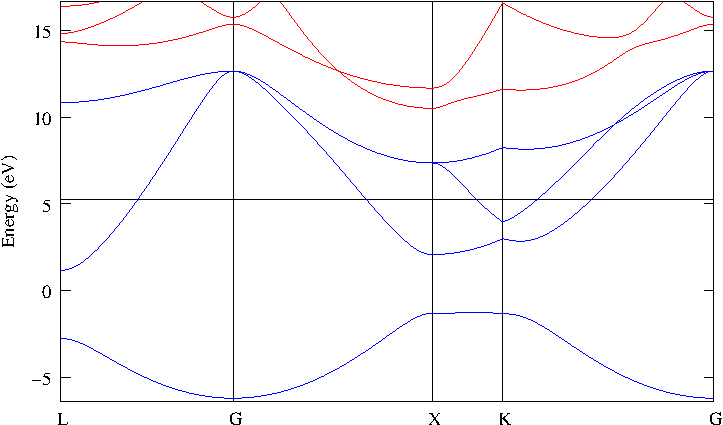
\includegraphics{lead}
\caption{Bandstructure of lead showing the position of the Fermi
  level. Only the lowest four bands are included in the calculation.} 
\label{fig:pb-bnd}
\end{center}
\end{figure}

\cleardoublepage


\section*{3: Silicon \tent{-- Disentangled MLWFs}}

\begin{itemize}
\item{Outline: \it{Obtain \tent{disentangled} MLWF for the valence and low-lying
    conduction states of Si. Plot the interpolated bandstructure}} 
\item{Generation Details: \it{From \pwscf, using norm-conserving
    pseudopotentials and a 4$\times$4$\times$4 k-point grid. Starting
    guess: atom-centred sp$^3$ hybrid orbitals}} 
\item{Directory: {\tt examples/example3/}}
\item{Input Files}
\begin{itemize}
\item{ {\tt silicon.win}  {\it The master input file}}
\item{ {\tt silicon.mmn}  {\it The overlap matrices $\Mkb$}}
\item{ {\tt silicon.amn}  {\it Projection $\Ak$ of the Bloch states onto a
    set of trial localised orbitals}} 
\item{ {\tt silicon.eig}  {\it The Bloch eigenvalues at each k-point}}
\end{itemize}
\end{itemize}
The valence and lower conduction states can be represented by MLWF
with $sp^3$-like symmetry. The lower conduction states are not 
separated from the higher states by an energy gap. In order to form
localised WF, we use the disentanglement procedure
introduced in Ref.~\cite{SMV}. The position of the inner and outer
energy windows are shown in Fig.~\ref{fig:si.bnd}. 
\begin{enumerate}
\item Run \wannier.
{\tt
\begin{quote}
wannier90.x silicon
\end{quote} }
Inspect the output file {\tt silicon.wout}. The minimisation of the
spread occurs in a two-step procedure~\cite{SMV}. First, we minimise
$\Omega_{\rm I}$ -- this is the extraction of the optimal subspace in
the disentanglement procedure. Then, we minimise $\Omega_{\rm D} +
\Omega_{{\rm OD}}$.

\item Plot the \sout{MLWF} \tent{energy bands} by adding the following
  commands to the input file {\tt silicon.win} {\tt
\begin{quote}
restart = plot

bands\_plot = true
\end{quote} }
and re-running \wannier. The files {\tt silicon\_band.dat} and {\tt
  silicon\_band.gnu} are created. 
To plot the bandstructure using gnuplot
\smallskip
{\tt
\begin{quote}
myshell> gnuplot

gnuplot> load `silicon\_band.gnu'
\end{quote} }
The k-point path for the bandstructure interpolation is set in the {\tt
  kpoint\_path} block. Try plotting along different paths. 
\end{enumerate}

\begin{figure}[h]
\begin{center}
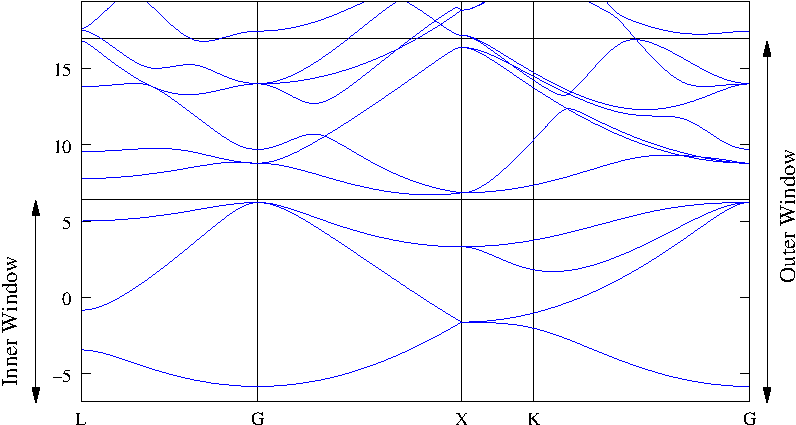
\includegraphics{si}
\caption{Bandstructure of silicon showing the position of the outer
  and inner energy windows.} 
\label{fig:si.bnd}
\end{center}
\end{figure}

\cleardoublepage


\section*{4: Copper \tent{-- Fermi surface, orbital character of
    energy bands}}

\begin{itemize}
\item{Outline: \it{Obtain MLWF to describe the states around the
    Fermi-level in copper}} 
\item{Generation Details: \it{From \pwscf, using ultrasoft
    pseudopotentials~\cite{USPP} and a
    4$\times$4$\times$4 k-point grid. Starting guess: five 
    atom-centred d orbitals, and two s orbitals centred on one of each
    of the two tetrahedral interstices.}}
\item{Directory: {\tt examples/example4/}}
\item{Input Files}
\begin{itemize}
\item{ {\tt copper.win}  {\it The master input file}}
\item{ {\tt copper.mmn}  {\it The overlap matrices $\Mkb$}}
\item{ {\tt copper.amn}  {\it Projection $\Ak$ of the Bloch states onto a
    set of trial localised orbitals}} 
\item{ {\tt copper.eig}  {\it The Bloch eigenvalues at each k-point}}
\end{itemize}

\end{itemize}

\begin{enumerate}
\item Run \wannier\ to minimise the MLWF spread
{\tt
\begin{quote}
wannier90.x copper
\end{quote} }
Inspect the output file {\tt copper.wout}. 

\item Plot the Fermi surface, it should look familiar! The Fermi
  energy is at 12.2103\,eV. 

\item Plot the interpolated bandstructure. A suitable path in k-space is
\smallskip
{\tt
\begin{quote}
begin kpoint\_path

G 0.00  0.00  0.00    X 0.50  0.50  0.00

X 0.50  0.50  0.00    W 0.50  0.75  0.25

W 0.50  0.75  0.25    L 0.00  0.50  0.00

L 0.00  0.50  0.00    G 0.00  0.00  0.00

G 0.00  0.00  0.00    K 0.00  0.50 -0.50
 
end kpoint\_path
\end{quote} }
\item Plot the contribution of the interstitial WF to the
  bandstructure. Add the following keyword to {\tt copper.win}
\smallskip
{\tt
\begin{quote}
bands\_plot\_project = 6,7
\end{quote} } The resulting file {\tt copper\_band\_proj.gnu} can be
opened with gnuplot. Red lines correspond to a large contribution from
the interstitial WF (blue line are a small contribution; ie a large
$d$ contribution).


\end{enumerate}




Investigate the effect of the outer and inner energy window on the
interpolated bands. 



\begin{figure}[h]
\begin{center}
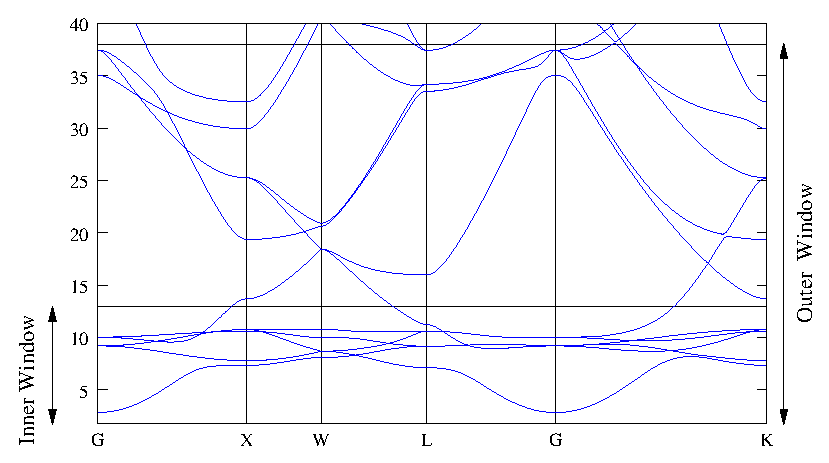
\includegraphics{cu}
\caption{Bandstructure of copper showing the position of the outer
  and inner energy windows.} 
\label{fig:cu-bnd}
\end{center}
\end{figure}

\cleardoublepage

\begin{center}
\Large{\bf Examples Using the {\sc pwscf} Interface}
\end{center}

The \pwscf\ plane-wave, density-functional theory code, which is
available as part of the \QE\ distribution ({\tt
  www.quantum-espresso.org}), is fully interfaced to \wannier\ via the
{\tt pw2wannier90} post-processing code that is also available as part
of \QE. The latest version of {\tt pw2wannier90} is included as part of 
the \wannier\ distribution. Please see the {\tt pwscf} directory for 
instructions on how to incorporate it into \pwscf. 

\textcolor{red}{Ivo: Should we explain somewhere in the tutorial
  (here?)  how to execute {\tt pw2wannier90} in parallel? (and also
  {\tt pw.x}) Note that in Example~16 Giovanni explained how to
  execute {\tt postw90} in parallel, and then I did the same for
  Examples~17--20. For 17--20 at least, running {\tt pw2wannier90} is
  even more time-consuming than running {\tt postw90}...}

\cleardoublepage

\section*{5: Diamond \tent{-- MLWFs for the valence bands}}
\begin{itemize}
\item{Outline: \it{Obtain MLWF for the valence bands of diamond}}
\item{Directory: {\tt examples/example5/}}
\item{Input Files}
\begin{itemize}
\item{ {\tt diamond.scf}  {\it The \pwscf\ input file for ground state
    calculation}} 
\item{ {\tt diamond.nscf}  {\it The \pwscf\ input file to obtain Bloch
    states on a uniform grid}} 
\item{ {\tt diamond.pw2wan}  {\it The input file for {\tt pw2wannier90}}}
\item{ {\tt diamond.win}  {\it The {\tt wannier90} input file}}
\end{itemize}
\end{itemize}

\begin{enumerate}
\item Run \pwscf\ to obtain the ground state of diamond\\
{\tt pw.x < diamond.scf > scf.out}

\item Run \pwscf\ to obtain the Bloch states on a uniform k-point grid\\
{\tt pw.x < diamond.nscf > nscf.out}

\item Run \wannier\ to generate a list of the required overlaps (written
  into the {\tt diamond.nnkp} file).\\ 
{\tt wannier90.x -pp diamond}

\item Run {\tt pw2wannier90} to compute the overlap between Bloch
  states and the projections for the starting guess (written in the
  {\tt diamond.mmn} and {\tt diamond.amn} files).\\  
{\tt pw2wannier90.x < diamond.pw2wan > pw2wan.out}

\item Run \wannier\ to compute the MLWF.\\
{\tt wannier90.x diamond}
\end{enumerate}

\cleardoublepage

\section*{6: Copper \tent{-- Fermi surface}}

\begin{itemize}
\item{Outline: \it{Obtain MLWF to describe the states around the
    Fermi-level in copper}}
\item{Directory: {\tt examples/example6/}}
\item{Input Files}
\begin{itemize}
\item{ {\tt copper.scf}  {\it The \pwscf\ input file for ground state
    calculation}} 
\item{ {\tt copper.nscf}  {\it The \pwscf\ input file to obtain Bloch states
    on a uniform grid}} 
\item{ {\tt copper.pw2wan}  {\it Input file for {\tt pw2wannier90}}}
\item{ {\tt copper.win}  {\it The {\tt wannier90} input file}}
\end{itemize}

\end{itemize}

\begin{enumerate}
\item Run \pwscf\ to obtain the ground state of copper\\
{\tt pw.x < copper.scf > scf.out}

\item Run \pwscf\ to obtain the Bloch states on a uniform k-point grid\\
{\tt pw.x < copper.nscf > nscf.out}

\item Run \wannier\ to generate a list of the required overlaps (written
  into the {\tt copper.nnkp} file).\\ 
{\tt wannier90.x -pp copper}

\item Run {\tt pw2wannier90} to compute the overlap between Bloch
  states and the projections for the starting guess (written in the
  {\tt copper.mmn} and {\tt copper.amn} files).\\  
{\tt pw2wannier90.x < copper.pw2wan > pw2wan.out}

\item Run \wannier\ to compute the MLWF.\\
{\tt wannier90.x copper}
\end{enumerate}

Inspect the output file {\tt copper.wout}. 

\begin{enumerate}
\item Use Wannier interpolation to obtain the Fermi surface of
  copper. Rather than re-running the whole calculation we can use the
  unitary transformations obtained in the first calculation and restart
  from the plotting routine. Add the following keywords to the {\tt
    copper.win} file:
{\tt
\begin{quote}
restart = plot

fermi\_energy = [insert your value here] 

fermi\_surface\_plot = true
\end{quote} }
and re-run \wannier. The value of the Fermi energy can be  
obtained from the initial first principles calculation. \wannier\
calculates the band energies, through wannier interpolation, on a
dense mesh of k-points in the Brillouin zone. The density of this grid is
controlled by the keyword {\tt fermi\_surface\_num\_points}. The default
value is 50 (i.e., 50$^3$ points).
The Fermi surface file {\tt copper.bxsf} can be viewed using XCrySDen,
e.g., 
{\tt
\begin{quote}
xcrysden --bxsf copper.bxsf
\end{quote} }


\item Plot the interpolated bandstructure. A suitable path in k-space is
\smallskip
{\tt
\begin{quote}
begin kpoint\_path

G 0.00  0.00  0.00    X 0.50  0.50  0.00

X 0.50  0.50  0.00    W 0.50  0.75  0.25

W 0.50  0.75  0.25    L 0.00  0.50  0.00

L 0.00  0.50  0.00    G 0.00  0.00  0.00

G 0.00  0.00  0.00    K 0.00  0.50 -0.50
 
end kpoint\_path
\end{quote} }
\end{enumerate}

\subsection*{Further ideas}
\begin{itemize}
\item Compare the Wannier interpolated bandstructure with the full
  \pwscf\ bandstructure. Obtain MLWF using a denser k-point grid.
\tent{{[Provide script for this? Link to Jonathan's URL?]}}
\item Investigate the effects of the outer and inner energy windows on
  the interpolated bands. 
\item Instead of extracting a subspace of seven states, we could
  extract a nine dimensional space (i.e., with $s$, $p$ and $d$
  character). Examine this case and compare the interpolated
  bandstructures.
\end{itemize}

%\begin{figure}[h]
%\begin{center}
%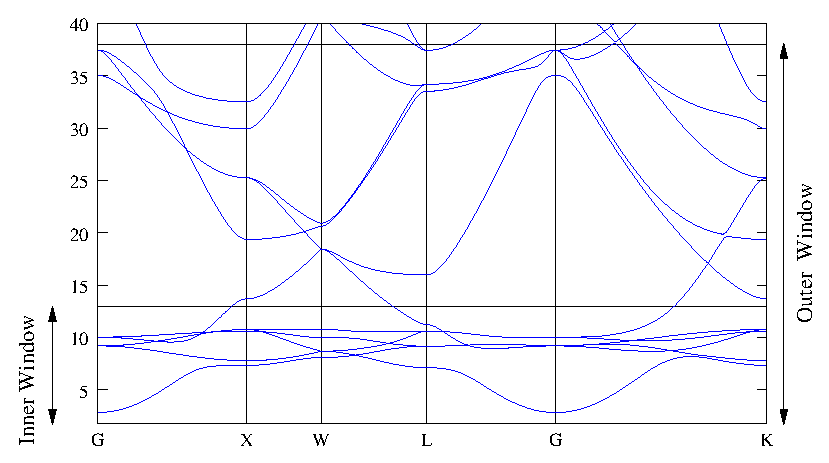
\includegraphics{cu}
%\caption{Band Structure of Copper showing the position of the outer
%  and inner energy windows.}
%\label{fig:cu-bnd}
%\end{center}
%\end{figure}

\cleardoublepage

\section*{7: Silane  (SiH$_4$) \tent{-- Molecular MLWFs using 
$\Gamma$-point sampling}}
\begin{itemize}
\item{Outline: \it{Obtain MLWF for the occupied states of molecular
    silane. $\Gamma$-point sampling}} 
\item{Directory: {\tt examples/example7/}}
\item{Input Files}
\begin{itemize}
\item{ {\tt silane.scf}  {\it The \pwscf\ input file for ground state
    calculation}} 
\item{ {\tt silane.nscf}  {\it The \pwscf\ input file to obtain Bloch states
    on a uniform grid}} 
\item{ {\tt silane.pw2wan}  {\it Input file for {\tt pw2wannier90}}}
\item{ {\tt silane.win}  {\it The {\tt wannier90} input file}}
\end{itemize}
\end{itemize}

\begin{enumerate}
\item Run \pwscf\ to obtain the ground state of silane\\
{\tt pw.x < silane.scf > scf.out}

\item Run \pwscf\ to obtain the Bloch states on a uniform k-point grid\\
{\tt pw.x < silane.nscf > nscf.out}

\item Run \wannier\ to generate a list of the required overlaps (written
  into the {\tt silane.nnkp} file).\\ 
{\tt wannier90.x -pp silane}

\item Run {\tt pw2wannier90} to compute the overlap between Bloch
  states and the projections for the starting guess (written in the
  {\tt silane.mmn} and {\tt silane.amn} files).\\  
{\tt pw2wannier90.x < silane.pw2wan > pw2wan.out}

\item Run \wannier\ to compute the MLWF.\\
{\tt wannier90.x silane}
\end{enumerate}

\cleardoublepage

\section*{8: Iron \tent{-- Spin-polarized WFs, total and projected DOS}}
\begin{itemize}
\item{Outline: \it{\sout{Obtain MLWF to describe the states around the
        Fermi-level in iron.} \tent{Generate Wannier functions for ferromagnetic
        iron, and use them to calculate the density of states (DOS) by Wannier
        interpolation.}}}
\item{Directory: {\tt examples/example8/}}
\item{Input Files}
\begin{itemize}
\item{ {\tt iron.scf}  {\it The \pwscf\ input file for ground state
    calculation}} 
\item{ {\tt iron.nscf}  {\it The \pwscf\ input file to obtain Bloch states
    on a uniform grid}} 
\item{ {\tt iron\_up.pw2wan}  {\it Input file for {\tt pw2wannier90} -
    spin up}} 
\item{ {\tt iron\_up.win} {\it The {\tt wannier90} \tent{and {\tt
          postw90}} input file - spin up}}
\item{ {\tt iron\_dn.pw2wan}  {\it Input file for {\tt pw2wannier90} -
    spin down}} 
\item{ {\tt iron\_dn.win}  {\it The {\tt wannier90} \tent{and {\tt
          postw90}} input file - spin down}}
\end{itemize}
\item{Note that we obtain the MLWF for spin up and spin down in
  separate calculations.} 
\end{itemize}

\begin{enumerate}
\item Run \pwscf\ to obtain the ground state of iron\\
{\tt pw.x < iron.scf > scf.out}

\item Run \pwscf\ to obtain the Bloch states on a uniform k-point grid\\
{\tt pw.x < iron.nscf > nscf.out}

\item Run \wannier\ to generate a list of the required overlaps (written
  into the {\tt iron\_up.nnkp} and {\tt iron\_dn.nnkp} files).\\
{\tt wannier90.x -pp iron\_up}\\
{\tt wannier90.x -pp iron\_dn}

\item Run {\tt pw2wannier90} to compute the overlap between Bloch
  states and the projections for the starting guess (written in the
  {\tt iron\_up.mmn}, {\tt iron\_dn.mmn}, {\tt iron\_up.amn} and {\tt
  iron\_dn.amn} files).\\ 
{\tt pw2wannier90.x < iron\_up.pw2wan > pw2wan.out}\\
{\tt pw2wannier90.x < iron\_dn.pw2wan > pw2wan.out}

\item Run \wannier\ to compute the MLWF.\\
{\tt wannier90.x iron\_up}\\
{\tt wannier90.x iron\_dn}

\item \tent{Compute the DOS on a $25\times 25 \times 25$ $k$-point grid. First add the following
lines to the two {\tt .win} input files,}
{\tt
\begin{quote}
dos = T

dos\_task = dos\_plot

dos\_interp\_mesh = 25
\end{quote}
}

\tent{and then run {\tt postw90},\\
{\tt postw90.x iron\_up}\\
{\tt postw90.x iron\_dn}
}

\item \tent{Plot the DOS with {\tt gnuplot}},
%
{\tt
\begin{quote}
myshell> gnuplot

gnuplot> plot `iron\_up\_dos.dat' u (-\$2):(\$1-12.6256) w l,`iron\_dn\_dos.dat' u 2:(\$1-12.6256) w l

\end{quote} 
}

\tent{We have set the zero of the energy scale at the Fermi level by
  subtracting %12.6256~eV,
  the value of the Fermi energy taken from {\tt scf.out}.  Check if
  the DOS is sufficiently well-converged by increasing the parameter
  {\tt dos\_interp\_mesh}.  }

\end{enumerate}

\tent{In the calculations above we chose $s$, $p$, and $d$-type trial
  orbitals (see {\tt .win} files),} {\tt
\begin{quote}
Fe:s;p;d

\end{quote}
}\tent{Let us analyze the evolution of the WFs during the
  gauge-selection step. Open one of the {\tt .wout} files and search
  for ``{\tt Initial state}''; those are the {\it projected} WFs. As
  expected they are atom-centered, with spreads organized in three
  groups, 1+3+5: one $s$, three $p$, and five $d$.  Now look at the
  final state at the end of the file.  The Wannier spreads have
  re-organized in two groups, 6+3; moreover, the six more diffuse WFs
  are now off-centered. The initial atomic-like orbitals hybridized
  with one another, becoming more localized in the process.}

\tent{To see when the hybridization took place, let us plot the
  evolution of the total spread~$\Omega$,} 
{\tt
\begin{quote}
myshell> grep SPRD iron\_up.wout >sprd\_up

myshell> gnuplot

gnuplot> plot `sprd\_up' u 6  w l

\end{quote}
}

\begin{figure}[h]
\begin{center}
\scalebox{0.4}{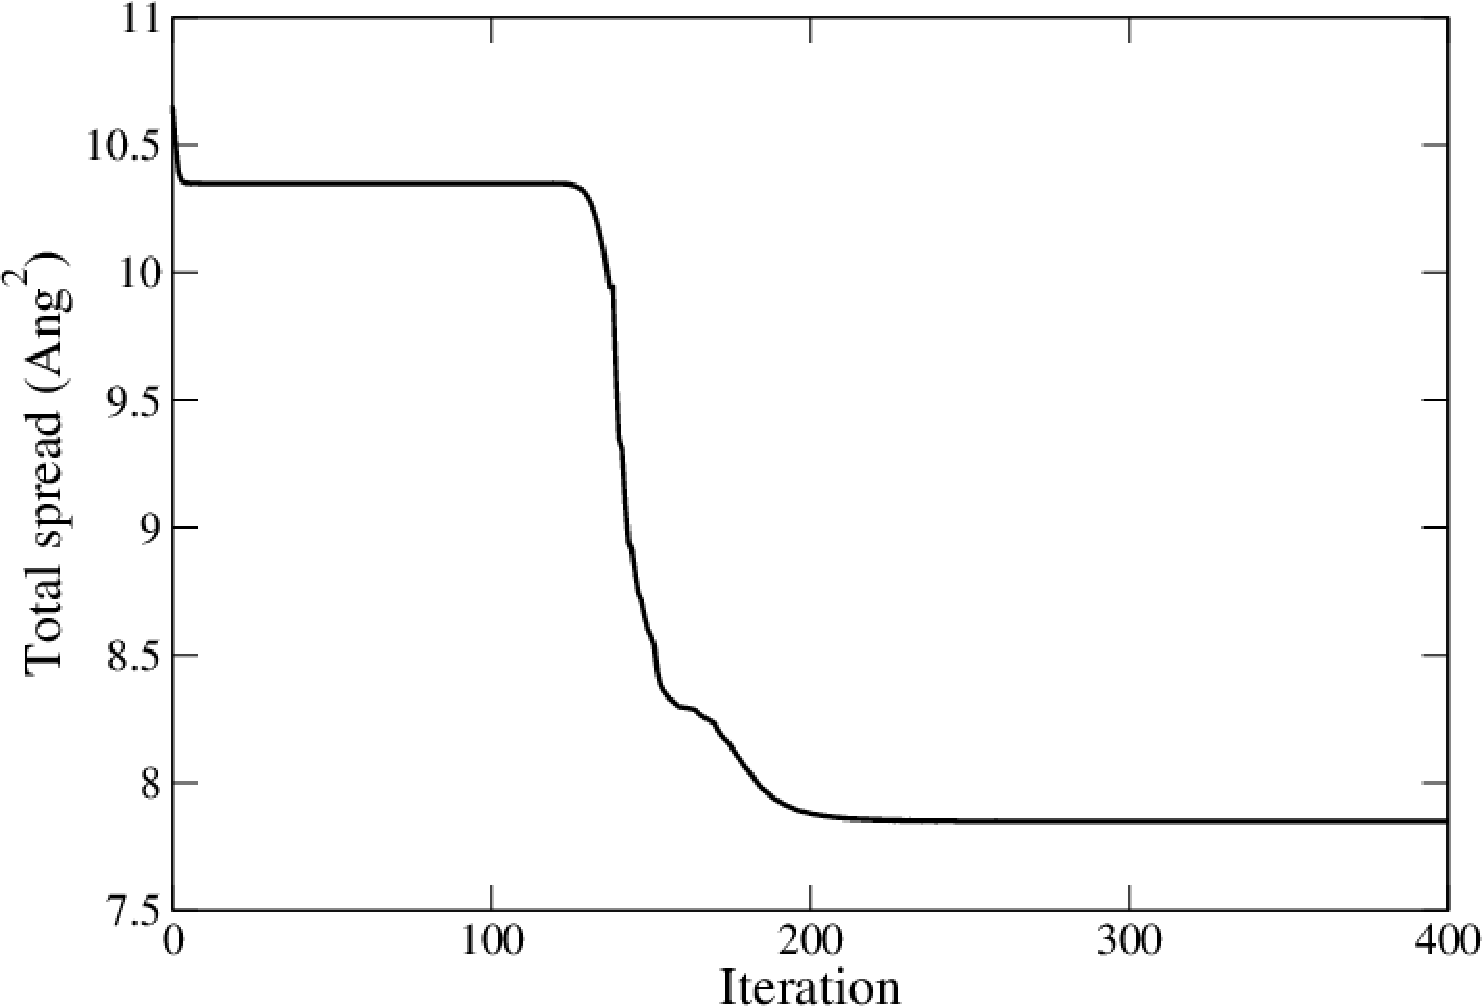
\includegraphics{Fe-spread}}
\caption{Evolution of the Wannier spread $\Omega$ of bcc Fe during the
  iterative minimization of the gauge-dependent part
  $\widetilde{\Omega}$, starting from $s$, $p$, and $d$-type trial
  orbitals.}
\label{fig:Fe-sprd}
\end{center}
\end{figure}


\tent{The first plateau corresponds to atom-centered WFs of separate
  $s$, $p$, and $d$ character, same as the trial orbitals, and the
  sharp drop at around iteration $120$ signals the onset of the
  hybridization. For more details, see Sec.~IV.B of
  Ref.~\cite{wang-prb06}. With hindsight, we can redo steps~4 and~5
  more efficiently using trial orbitals with the same character as the
  final MLWFs,} {\tt
\begin{quote}
Fe:sp3d2;dxy;dxz,dyz
\end{quote}
}


\tent{Physical quantities should come out essentially the same
  computed with any reasonable set of localized WFs, not necessarily
  maximally-localized.  Let us re-run steps~4 and~5 again starting
  from $s$, $p$, and $d$-type trial orbitals, but stopping the
  minimization of $\widetilde{\Omega}$ before the onset of
  hybridization,} {\tt
\begin{quote}
num\_iter = 50
\end{quote}
}

\tent{Now recalculate the DOS, and check that it is almost identical to
  the one computed earlier using the hybridized set of MLWFs.}


\subsection*{Further ideas}

[In the following it is assumed that {\it non-hybridized} WFs of
separate $s$, $p$, and $d$ character have been obtained as described
above.]

\begin{itemize}

\item \tent{In order to obtain the DOS projected onto the $p$-type
    WFs, add to the {\tt .win} files the lines} {\tt
\begin{quote}
dos\_project = 2,3,4
\end{quote}
}

(compare with Example~4)
and re-run {\tt postw90}. Plot the $p$-projected DOS for both up- and
down-spin bands. Repeat for the $s$ and and $d$ projections.

\item \tent{Re-run {\tt wannier90} after adding to the {\tt .win}
    files the instruction} {\tt
\begin{quote}
write\_hr\_diag = T
\end{quote}
}

\tent{This tells {\tt wannier90} to write in the output file the
  diagonal (``on-site'') Wannier matrix elements of the
  Hamiltonian. The difference between corresponding values in {\tt
    iron\_up.wout} and in {\tt iron\_dn.wout} gives the exchange
  splittings for the individual $s$, $p$, and $d$-type WFs. Compare
  their magnitudes with the splittings displayed by the total and
  orbital-projected DOS.}

\end{itemize}

\cleardoublepage


\section*{9: Cubic BaTiO$_3$}
\begin{itemize}
\item{Outline: \it{Obtain MLWF for a perovskite}}
\item{Directory: {\tt examples/example9/}}
\item{Input Files}
\begin{itemize}
\item{ {\tt batio3.scf}  {\it The \pwscf\ input file for ground state
    calculation}} 
\item{ {\tt batio3.nscf}  {\it The \pwscf\ input file to obtain Bloch states
    on a uniform grid}} 
\item{ {\tt batio3.pw2wan}  {\it Input file for {\tt pw2wannier90}}}
\item{ {\tt  batio3.win}  {\it The {\tt wannier90} input file}}
\end{itemize}
\end{itemize}

 To start with, we are going to obtain MLWF for the oxygen 2p
  states. From the bandstructure~\cite{BaTiO3}, these form an isolated
  group of bands. We use the \wannier\ keyword {\tt exclude\_bands} to
  remove all but the 2p bands from the calculation of the overlap
  and projection matrices (we don't have to do this, but it saves time).

\begin{enumerate}
\item Run \pwscf\ to obtain the ground state of BaTiO$_3$\\
{\tt pw.x < BaTiO3.scf > scf.out}

\item Run \pwscf\ to obtain the Bloch states on a uniform k-point grid\\
{\tt pw.x < BaTiO3.nscf > nscf.out}

\item Run \wannier\ to generate a list of the required overlaps (written
  into the {\tt BaTiO3.nnkp} file).\\ 
{\tt wannier90.x -pp BaTiO3}

\item Run {\tt pw2wannier90} to compute the overlap between Bloch
  states and the projections for the starting guess (written in the
  {\tt BaTiO3.mmn} and {\tt BaTiO3.amn} files).\\  
{\tt pw2wannier90.x < BaTiO3.pw2wan > pw2wan.out}

\item Run \wannier\ to compute the MLWF.\\
{\tt wannier90.x BaTiO3}
\end{enumerate}

Inspect the output file {\tt BaTiO3.wout}. 

Plot the second MLWF, as described in Section~1, by adding the
following keywords to the input file {\tt BaTiO3.win}
{\tt
\begin{quote}
wannier\_plot = true\\
restart = plot\\
wannier\_plot\_list = 2\\
wannier\_plot\_supercell = 3
\end{quote} }
and re-running \wannier. Visualise it using XCrySDen,
{\tt
\begin{quote}
xcrysden --xsf BaTiO3\_00002.xsf
\end{quote} }

We can now simulate the ferroelectric phase by displacing the Ti
  atom. Change its position to 
{\tt
\begin{quote}
Ti 0.505 0.5 0.5
\end{quote}
}
and regenerate the MLWF (i.e., compute the ground-state charge
density and Bloch states using \pwscf, etc.) and look at the change in
the second MLWF.

\subsection*{Further ideas}
\begin{itemize}
\item Look at MLWF for other groups of bands. What happens if you form
  MLWF for the whole valence manifold?

\item Following Ref.~\cite{BaTiO3}, compute the Born effective charges from the
  change in Wannier centres under an atomic displacement. 
\end{itemize}

\cleardoublepage

\section*{10: Graphite}
\begin{itemize}
\item{Outline: \it{Obtain MLWF for graphite (AB, Bernal)}}
\item{Directory: {\tt examples/example10/}}
\item{Input Files}
\begin{itemize}
\item{ {\tt graphite.scf}  {\it The \pwscf\ input file for ground
    state calculation}} 
\item{ {\tt graphite.nscf}  {\it The \pwscf\ input file to obtain Bloch
    states on a uniform grid}} 
\item{ {\tt graphite.pw2wan}  {\it Input file for {\tt pw2wannier90}}}
\item{ {\tt graphite.win}  {\it The {\tt wannier90} input file}}
\end{itemize}
\end{itemize}

\begin{enumerate}
\item Run \pwscf\ to obtain the ground state of graphite\\
{\tt pw.x < graphite.scf > scf.out}

\item Run \pwscf\ to obtain the Bloch states on a uniform k-point grid\\
{\tt pw.x < graphite.nscf > nscf.out}

\item Run \wannier\ to generate a list of the required overlaps (written
  into the {\tt graphite.nnkp} file).\\ 
{\tt wannier90.x -pp graphite}

\item Run {\tt pw2wannier90} to compute the overlap between Bloch
  states and the projections for the starting guess (written in the
  {\tt graphite.mmn} and {\tt graphite.amn} files).\\  
{\tt pw2wannier90.x < graphite.pw2wan > pw2wan.out}

\item Run \wannier\ to compute the MLWF.\\
{\tt wannier90.x graphite}
\end{enumerate}


\cleardoublepage


\section*{11: Silicon \tent{-- Valence and conduction states, scissors correction}}
\subsection*{Valence States}
\begin{itemize}
\item{Outline: \it{Obtain MLWF for the valence bands of silicon.}}
\item{Directory: {\tt examples/example11/}}
\item{Input Files}
\begin{itemize}
\item{ {\tt silicon.scf}  {\it The \pwscf\ input file for ground state
    calculation}} 
\item{ {\tt silicon.nscf}  {\it The \pwscf\ input file to obtain Bloch
    states on a uniform grid}} 
\item{ {\tt silicon.pw2wan}  {\it Input file for {\tt pw2wannier90}}}
\item{ {\tt silicon.win}  {\it The {\tt wannier90} input file}}
\end{itemize}

\end{itemize}

\begin{enumerate}
\item Run \pwscf\ to obtain the ground state of silicon\\
{\tt pw.x < silicon.scf > scf.out}

\item Run \pwscf\ to obtain the Bloch states on a uniform k-point
  grid. Note that we request the lower 4 (valence) bands\\ 
{\tt pw.x < silicon.nscf > nscf.out}

\item Run \wannier\ to generate a list of the required overlaps (written
  into the {\tt silicon.nnkp} file).\\
{\tt wannier90.x -pp silicon}

\item Run {\tt pw2wannier90} to compute the overlap between Bloch
  states and the projections for the starting guess (written in the
  {\tt silicon.mmn} and {\tt  silicon.amn} files).\\
{\tt pw2wannier90.x < silicon.pw2wan > pw2wan.out}

\item Run \wannier\ to compute the MLWF.\\
{\tt wannier90.x silicon}

\end{enumerate}

Inspect the output file {\tt silicon.wout}. The total spread converges to its
minimum value after just a few iterations. Note that the geometric centre of
each MLWF lies at the centre of the Si-Si bond.
Note also that the memory requirement for the minimisation of
the spread is very low as the MLWF are defined 
by just the 4$\times$4 unitary matrices $\Uk$. 

Plot the MLWF by adding the following keywords to the input file {\tt
  silicon.win} 
{\tt
\begin{quote}
wannier\_plot = true
\end{quote} }
and re-running \wannier. Visualise them using XCrySDen, e.g.,
{\tt
\begin{quote}
xcrysden --xsf silicon\_00001.xsf
\end{quote} }

\subsection*{Valence + Conduction States}

\begin{itemize}
\item{Outline: \it{Obtain MLWF for the valence and low-lying
      conduction-band states of Si. Plot the interpolated
      bandstructure. \tent{Apply a scissors correction to the
        conduction bands.}}}
\item{Input Files}
\begin{itemize}
\item{ {\tt silicon.scf}  {\it The \pwscf\ input file for ground state
    calculation}} 
\item{ {\tt silicon.nscf}  {\it The \pwscf\ input file to obtain Bloch
    states on a uniform grid}} 
\item{ {\tt silicon.pw2wan}  {\it Input file for {\tt pw2wannier90}}}
\item{ {\tt silicon.win}  {\it The {\tt wannier90} input file}}
\end{itemize}
\end{itemize}
The valence and lower conduction states can be represented by MLWF
with $sp^3$-like symmetry. The lower conduction states are not 
separated by an energy gap from the higher states. In order to form
localised WF we use the disentanglement procedure
introduced in Ref.~\cite{SMV}. The position of the inner and outer
energy windows are shown in Fig.~\ref{fig:si.bnd}. 
\begin{enumerate}
\item Modify the input file and run \pwscf\ and \wannier.\\
Inspect the output file {\tt silicon.wout}. The minimisation of the
spread occurs in a two-step procedure. First, we minimise $\Omega_{\rm
  I}$ -- this is the extraction of the optimal subspace in the 
disentanglement procedure. Then, we minimise $\Omega_{\rm
  O}+\Omega_{{\rm OD}}$.

\item Plot the bandstructure by adding the following commands to the
 input file {\tt silicon.win}
{\tt
\begin{quote}
restart = plot

bands\_plot = true
\end{quote} }
and re-running \wannier. The files {\tt silicon\_band.dat} and {\tt
  silicon\_band.gnu} are created. To plot the bandstructure using
  gnuplot \smallskip
{\tt
\begin{quote}
myshell> gnuplot

gnuplot> load `silicon\_band.gnu'
\end{quote} }
The k-point path for the bandstructure interpolation is set in the {\tt
  kpoint\_path} block. Try plotting along different paths. 

\item \tent{Shift the conduction bands upwards in energy by
    0.65~eV. This {\it ad-hoc} ``scissors correction'' is applied to
    the Hamiltonian in the Wannier basis using the instructions}
%
{\tt
\begin{quote}
num\_valence\_bands = 4

scissors\_shift = 0.65
\end{quote} }
%
\tent{Plot together the original and scissors-corrected bands.}

\end{enumerate}

\subsection*{Further ideas}

\begin{itemize}
\item Compare the Wannier interpolated bandstructure with the full
  \pwscf\ bandstructure. Compute MLWF using a finer
  k-point grid (e.g., 6$\times$6$\times$6 or 8$\times$8$\times$8) and
  note how the accuracy of the interpolation increases~\cite{WanInt}.
\item Compute four MLWF spanning the low-lying conduction states (see
  Ref.~\cite{SMV}).
\end{itemize}

%\begin{figure}[h]
%\begin{center}
%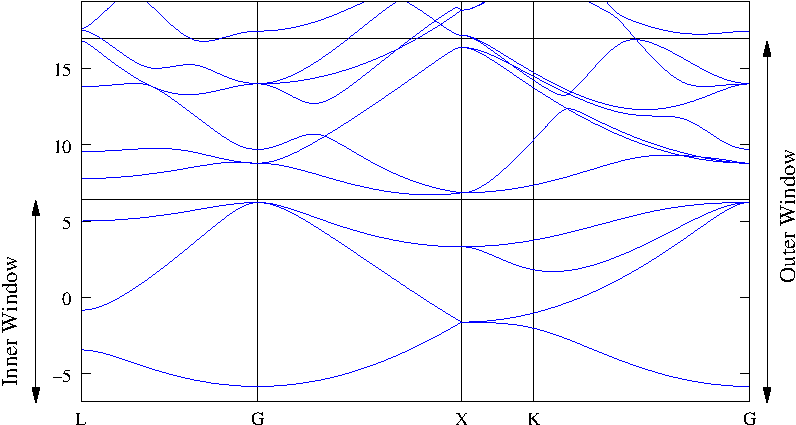
\includegraphics{si}
%\caption{Band Structure of Silicon showing the position of the outer
%and inner energy windows.}
%\label{fig:si.bnd}
%\end{center}
%\end{figure}

\cleardoublepage


\section*{12: Benzene}
\subsection*{Valence States}
\begin{itemize}
\item{Outline: \it{Obtain MLWF for the valence states of benzene}}
\item{Directory: {\tt examples/example12/}}
\item{Input Files}
\begin{itemize}
\item{ {\tt benzene.scf}  {\it The \pwscf\ input file for ground state
    calculation}} 
\item{ {\tt benzene.pw2wan}  {\it Input file for {\tt pw2wannier90}}}
\item{ {\tt benzene.win}  {\it The {\tt wannier90} input file}}
\end{itemize}

\end{itemize}

\begin{enumerate}
\item Run \pwscf\ to obtain the ground state of benzene\\
{\tt pw.x < benzene.scf > scf.out}

\item Run \wannier\ to generate a list of the required overlaps (written
  into the {\tt benzene.nnkp} file).\\
{\tt wannier90.x -pp benzene}

\item Run {\tt pw2wannier90} to compute the overlap between Bloch
  states and the projections for the starting guess (written in the
  {\tt benzene.mmn} and {\tt  benzene.amn} files).\\
{\tt pw2wannier90.x < benzene.pw2wan > pw2wan.out}

\item Run \wannier\ to compute the MLWF.\\
{\tt wannier90.x benzene}

\end{enumerate}

Inspect the output file {\tt benzene.wout}. The total spread converges
to its minimum value after just a few iterations. 

Plot the MLWF by adding the following keywords to the input file {\tt
  benzene.win} 
{\tt
\begin{quote}
restart               = plot\\
wannier\_plot         = true\\
wannier\_plot\_format = cube\\
wannier\_plot\_list   = 2-4
\end{quote} }
and re-running \wannier. Visualise them using, e.g., XCrySDen. 

\subsection*{Valence + Conduction States}

\begin{itemize}
\item{Outline: \it{Obtain MLWF for the valence and low-lying
    conduction states of benzene.}} 
\item{Input Files}
\begin{itemize}
\item{ {\tt benzene.scf}  {\it The \pwscf\ input file for ground state
    calculation}} 
\item{ {\tt benzene.nscf}  {\it The \pwscf\ input file to obtain Bloch
    states for the conduction states}} 
\item{ {\tt benzene.pw2wan}  {\it Input file for {\tt pw2wannier90}}}
\item{ {\tt benzene.win}  {\it The {\tt wannier90} input file}}
\end{itemize}
\end{itemize}
In order to form localised WF we use the disentanglement
procedure. The position of the inner energy window is set to lie in
the energy gap; the outer energy window is set to 4.0\,eV. Modify the
input file appropriately. 
\begin{enumerate}
\item Run \pwscf\ and \wannier.\\
Inspect the output file {\tt benzene.wout}. The minimisation of the
spread occurs in a two-step procedure. First, we minimise $\Omega_{\rm
  I}$. Then, we minimise $\Omega_{\rm O}+\Omega_{{\rm OD}}$.

\item Plot the MLWF by adding the following commands to the
 input file {\tt benzene.win}
{\tt
\begin{quote}
restart               = plot\\
wannier\_plot         = true\\
wannier\_plot\_format = cube\\
wannier\_plot\_list   = 1,7,13
\end{quote} }
and re-running \wannier. Visualise them using, e.g., XCrySDen. 
\end{enumerate}

\cleardoublepage

\section*{13: (5,5) Carbon Nanotube \tent{-- Transport properties}}
%\subsection*{Transport properties}

\begin{itemize}
  \item{Outline: \it{Obtain the bandstructure, quantum conductance and
  density of states of a metallic (5,5) carbon nanotube}}
  \item{Directory: {\tt examples/example13/}}
  \item{Input Files}
    \begin{itemize}
      \item{ {\tt cnt55.scf}  {\it The \pwscf\ input file for ground state
	  calculation}}
      \item{ {\tt cnt55.nscf}  {\it The \pwscf\ input file to obtain Bloch
	  states for the conduction states}} 
      \item{ {\tt cnt55.pw2wan}  {\it Input file for {\tt pw2wannier90}}}
      \item{ {\tt cnt55.win}  {\it The {\tt wannier90} input file}}
    \end{itemize}
\end{itemize}

In order to form localised WF that describe both the occupied and
unoccupied $\pi$ and $\pi^{\ast}$ manifolds, we use the
disentanglement procedure to extract a smooth manifold of states that
has dimension equal to 2.5 times the number of carbon atoms per unit
cell~\cite{WanTran}. The positions of the energy windows are shown in
Fig.~\ref{fig:cnt.win}.

The part of the \wannier\ input file that controls the transport part
of the calculation looks like:

{\tt
\begin{quote}
transport                 = true\\
transport\_mode           = bulk\\
one\_dim\_axis            = z\\
dist\_cutoff              =  5.5\\
fermi\_energy             = -1.06\\
tran\_win\_min            = -6.5\\
tran\_win\_max            = 6.5\\
tran\_energy\_step         = 0.01\\
dist\_cutoff\_mode        = one\_dim\\
translation\_centre\_frac = 0.0 0.0 0.0
\end{quote} }

Descriptions of these and other keywords related to the calculation of
transport properties can be found in the User Guide.

\begin{enumerate}
\item Run \pwscf\ and \wannier.\\
Inspect the output file {\tt cnt55.wout}. The minimisation of the
spread occurs in a two-step procedure. First, we minimise $\Omega_{\rm
  I}$. Then, we minimise $\Omega_{\rm O}+\Omega_{{\rm OD}}$.
\item Note that the initial $p_{z}$ projections on the carbon atoms
are oriented in the radial direction with respect to the nanotube
axis.
\item The interpolated bandstructure is written to {\tt
cnt55\_band.agr} (since {\tt bands\_plot\_format = xmgr} in the input
file).
\item The quantum conductance and density of states are written to the
files {\tt cnt55\_qc.dat} and {\tt cnt55\_dos.dat}, respectively. 
Note that this part of the calculation may take some time. You can 
follow its progress by monitoring the output to these files. 
Use a package such as {\tt gnuplot} or {\tt xmgrace} in order to visualise
the data. You should get something that looks like Fig.~\ref{fig:cnt.tran}.
\end{enumerate}

\begin{figure}[h]
\begin{center}
\scalebox{0.75}{\includegraphics{cnt_win}}
\caption{Bandstructure of (5,5) carbon nanotube showing the position
  of the outer and inner energy windows.}
\label{fig:cnt.win}
\end{center}
\end{figure}

\begin{figure}[h]
\begin{center}
\scalebox{0.8}{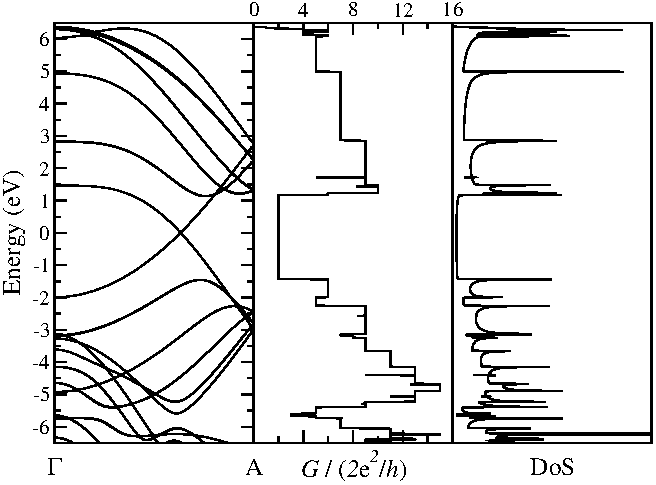
\includegraphics{cnt_tran}}
\caption{Wannier interpolated bandstructure, quantum conductance and
density of states of (5,5) carbon nanotube. Note that the Fermi level has been shifted 
by 1.06eV with respect to Fig.~\ref{fig:cnt.win}.}
\label{fig:cnt.tran}
\end{center}
\end{figure}

\cleardoublepage

\section*{14: Linear Sodium Chain \tent{-- Transport properties}}

\begin{itemize}
  \item{Outline: \it{Compare the quantum conductance of a periodic 
  	linear chain of Sodium atoms with that of a defected chain}}
  \item{\begin{tabbing}
  Directories: \= {\tt examples/example14/periodic}\\ 
    				 \> {\tt examples/example14/defected}
    		\end{tabbing}}
  \item{Input Files}
    \begin{itemize}
      \item{ {\tt Na\_chain.scf}  {\it The \pwscf\ input file for ground state
	  calculation}}
      \item{ {\tt Na\_chain.nscf}  {\it The \pwscf\ input file to obtain Bloch
	  states for the conduction states}} 
      \item{ {\tt Na\_chain.pw2wan}  {\it Input file for {\tt pw2wannier90}}}
      \item{ {\tt Na\_chain.win}  {\it The {\tt wannier90} input file}}
    \end{itemize}
\end{itemize}

The periodic system contains two unit cells evenly distributed along
the supercell. Transport calculations are performed using {\tt
  transport\_mode = bulk} and so the resulting quantum conductance
represents that of an infinite periodic chain.

The part of the \wannier\ input file that controls the transport part
of the calculation looks like:

{\tt
\begin{quote}
transport = true\\
transport\_mode = bulk\\
tran\_read\_ht = false\\
one\_dim\_axis = x\\
fermi\_energy = -2.7401\\
tran\_win\_min = -5.0\\
tran\_win\_max = 5.0\\
tran\_energy\_step = 0.01\\
translation\_centre\_frac = 0.5 0.5 0.5\\
tran\_num\_bb = 2

\end{quote} }

The defected system uses a 13 atom supercell with the central atom
position altered to break symmetry. Setting {\tt transport\_mode = lcr} with tell 
\wannier\ to treat the system as an infinte sytsem with the defect at its centre.
The supercell is chosen so that is conforms to the 2c2 geometry (see User Guide 
for details). Each principal layer is 2 atoms long so that the conductor 
region contains the defected atom plus a single atom on either side.

The transport section of the input file contians  these key differences:

{\tt
\begin{quote}
transport\_mode = lcr\\
tran\_num\_ll = 2\\
tran\_num\_cell\_ll = 2\\

\end{quote} }

Descriptions of these and other keywords related to the calculation of
transport properties can be found in the User Guide.

\begin{enumerate}
\item Run \pwscf\ and \wannier\ for the periodic system.
\item Run \pwscf\ and \wannier\ for the defected system.
\item The quantum conductance is written to the files {\tt periodic/Na\_chain\_qc.dat} 
and \linebreak{\tt defected/Na\_chain\_dos.dat}, respectively. 
Compare the quantum conductance of the periodic (bulk) calculation with the
defected (LCR) calculation. Your plot should look like Fig.~\ref{fig:Na_qc}.
\end{enumerate}


\begin{figure}[h]
\begin{center}
\scalebox{0.3}{\includegraphics{Na_qc}}
\caption{Quantum conductance of periodic Sodium chain (black) compared to that of the defected Sodium chain (red).}
\label{fig:Na_qc}
\end{center}
\end{figure}

\cleardoublepage

\section*{15: (5,0) Carbon Nanotube}

\emph{Note that these systems require reasonably large-scale electronic 
structure calculations.}

\subsection*{Bulk Transport properties}

\begin{itemize}
  \item{Outline: \it{Obtain the quantum conductance of a pristine single-walled carbon nanotube}}
  \item{Directory: {\tt examples/example14/periodic}}
  \item{Input Files}
    \begin{itemize}
      \item{ {\tt cnt.scf}  {\it The \pwscf\ input file for ground state
	  calculation}}
      \item{ {\tt cnt.nscf}  {\it The \pwscf\ input file to obtain Bloch
	  states for the conduction states}} 
      \item{ {\tt cnt.pw2wan}  {\it Input file for {\tt pw2wannier90}}}
      \item{ {\tt cnt.win}  {\it The {\tt wannier90} input file}}
    \end{itemize}
\end{itemize}


First we consider a single unit cell, with 10 k-points. With 
{\tt transport\_mode = bulk} we compute the transport properties 
of a pristine, infinite, periodic (5,0) carbon nanotube. Later, we will 
compare the quantum conductance of this system with a defected
nanotube.

\begin{enumerate}
\item Run \pwscf\ and \wannier.\\ 
\item The quantum conductance and density of states are written to the
files {\tt cnt\_qc.dat} and {\tt cnt\_dos.dat}, respectively.
\end{enumerate}

\subsection*{LCR transport properties -- Defected nanotube}

\begin{itemize}
  \item{Outline: \it{Use the automated LCR routine to investigate the effect of
  a single silicon atom in a infinite (5,0) carbon nanotube.}}
  \item{Directory: {\tt examples/example15/defected}}
  \item{Input Files}
    \begin{itemize}
      \item{ {\tt cnt+si.scf}  {\it The \pwscf\ input file for ground state
	  calculation}}
      \item{ {\tt cnt+si.nscf}  {\it The \pwscf\ input file to obtain Bloch
	  states for the conduction states}} 
      \item{ {\tt cnt+si.pw2wan}  {\it Input file for {\tt pw2wannier90}}}
      \item{ {\tt cnt+si.win}  {\it The {\tt wannier90} input file}}
    \end{itemize}
\end{itemize}

In this calculation an 11-atom supercell is used with a single silicon
substitutional defect in the central unit cell. The supercell is
chosen so that is conforms to the 2c2 geometry (see User Guide for
details) with principal layers set to be two unit cells long.

\begin{enumerate}
\item Run \pwscf\ and \wannier. Again these are large calculations, progress
can be monitored by viewing respective output files.\\
\item The quantum conductance is written to {\tt cnt+si\_qc.dat}. 
Compare the quantum conductance with the periodic (bulk) calculation.
Your plot should look like Fig.~\ref{fig:cnt_qc}.

\end{enumerate}

\begin{figure}[h]
\begin{center}
\scalebox{0.3}{\includegraphics{cnt_qc}}
\caption{Quantum conductance of infinite pristine nanotube (black) 
compared to that of the infinite nanotube with the substitutional silicon 
defect (red).}
\label{fig:cnt_qc}
\end{center}
\end{figure}

\subsection*{Further ideas}
\begin{itemize}
\item Set {\tt hr\_plot = true} in the bulk case. Consider the magnitude of Hamiltonian 
	elements between Wannier functions in increasingly distant unit cells. Are two 
	unit cell principal layers really large enough, or are significant errors introduced?
\item Does one unit cell either side of the defected unit cell shield the disorder
	so that the leads are ideal? Does the quantum conductance change if these 
	`buffer' regions are increased?
\end{itemize}

\cleardoublepage

\section*{16: Silicon -- Boltzmann transport}
\begin{itemize}
\item{Outline: \it{Obtain MLWF for the valence and low-lying
    conduction states of Si. Calculate the electrical conductivity, the
    Seebeck coefficient and the thermal conductivity in the constant
    relaxation time approximation using the \bw\ module.}} 
\item{Directory: {\tt examples/example16/}}
\item{Input Files}
\begin{itemize}
\item{ {\tt Si.scf}  {\it The \pwscf\ input file for ground state
    calculation}} 
\item{ {\tt Si.nscf}  {\it The \pwscf\ input file to obtain Bloch
    states on a uniform grid}} 
\item{ {\tt Si.pw2wan}  {\it Input file for {\tt pw2wannier90}}}
\item{ {\tt Si.win}  {\it The \wannier\ and \postw\ input file}}
\end{itemize}

\end{itemize}

Note the first five steps in the following are the same of Example~11.
If you have already run Example~11 (in particular, the section ``\emph{Valence + Conduction States}'')
you can start from those files and continue from point 6, after adding the \bw\ flags to the
input file.
\begin{enumerate}
\item Run \pwscf\ to obtain the ground state of silicon\\
{\tt pw.x < Si.scf > scf.out}

\item Run \pwscf\ to obtain the Bloch states on a uniform k-point
  grid. Details on the disentanglement procedure are discussed in Example~11.\\ 
{\tt pw.x < Si.nscf > nscf.out}

\item Run \wannier\ to generate a list of the required overlaps (written
  into the {\tt Si.nnkp} file).\\
{\tt wannier90.x -pp Si}

\item Run {\tt pw2wannier90} to compute the overlap between Bloch
  states and the projections for the starting guess (written in the
  {\tt Si.mmn} and {\tt  Si.amn} files).\\
{\tt pw2wannier90.x < Si.pw2wan > pw2wan.out}

\item Run \wannier\ to compute the MLWF.\\
{\tt wannier90.x Si}

\item Run \postw\ to calculate the transport coefficients.\\
For serial execution use: {\tt postw90.x Si}  \\
For parallel execution use: {\tt mpirun -np 8 postw90.x Si} \\
Note that the {\tt mpirun} command-line flags may be different in your MPI implementation: read your MPI manual. You may also want to change the number of processors (8 in this example).

\end{enumerate}

Inspect the output file {\tt Si.wout} and check if the convergence was reached both in the
disentanglement and in the wannierisation steps (as discussed in further detail in Example~11).
You may also want to plot the Wannier functions and the interpolated band structure.

Inspect the output file {\tt Si.wpout}. It summarizes the main details of the calculation (more details can be obtained by setting a larger value of the \verb#iprint# flag). 
Check if no warnings are issued. Note that if no special flags are passed to \bw, it assumes that
the ab-initio calculation did not include magnetization effects, and thus it sets to 2 the
number of electrons per state.

Note also that the value of the relaxation time $\tau=10$~fs in the
example is set only as an \sout{exemplificative} \tent{representative}
value; note also that only the electrical and thermal conductivity
depend on $\tau$, while the Seebeck coefficient is independent of
$\tau$.

Using your favourite plotting program, plot the {\tt Si\_boltzdos.dat} file to inspect the DOS.

Using your favourite plotting program, plot columns 1 and 3 of the {\tt Si\_seebeck.dat} file to inspect the $S_{xx}$ component of the Seebeck coefficient as a function of the chemical potential $\mu$, at $T=300$~K.

\subsection*{Further ideas}

\begin{itemize}
\item Change the interpolation to a $60\times 60\times 60$ mesh and run again \postw\ to check if the results for the transport properties are converged. 

\item Change the {\tt Si.win} input file so that it calculates the transport coefficients for temperatures from 300 to 700~K, with steps of 200~K. Rerun \postw\ and verify that the increase in execution time is neglibile (in fact, most of the time is spent to interpolate the band structure on the $k$ mesh).

Plot the Seebeck coefficient for the three temperatures $T=300$~K, $T=500$~K and $T=700$~K. To do this, you have to filter the {\tt Si\_seebeck.dat} to select only those lines where the second column is equal to the required temperature. A possible script to select the $S_{xx}$ component of the Seebeck coefficient for $T=500$~K using the {\tt awk/gawk} command line program is the following:
\begin{verbatim}
awk `{if ($2 == 500) {print $1, $3;}}' < Si_seebeck.dat \
    > Si_seebeck_xx_500K.dat
\end{verbatim}
Then, you can plot columns 1 and 2 of the output file \verb#Si_seebeck_xx_500K.dat#.
\item Try to calculate the Seebeck coefficient as a function of the temperature, for a $n-$doped sample with, e.g., $n=10^{18}$ cm$^{-3}$. Note that to this aim, you need to calculate consistently the value $\mu(T)$ of the chemical potential as a function of the temperature, so as to reproduce the given value of $n$. Then, you have to write a small program/script to interpolate the output of \bw, that you should have run on a suitable grid of $(\mu,T)$ points.
\end{itemize}

%\begin{figure}[h]
%\begin{center}
%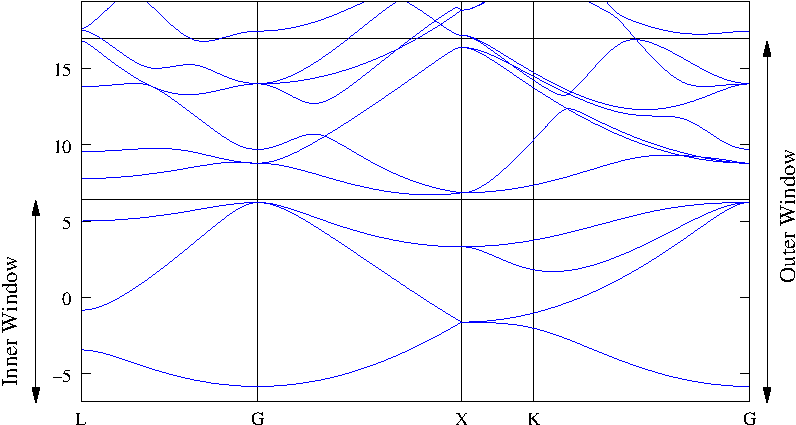
\includegraphics{si}
%\caption{Band Structure of Silicon showing the position of the outer
%and inner energy windows.}
%\label{fig:si.bnd}
%\end{center}
%\end{figure}

\cleardoublepage


\section*{17: Iron -- Spin-orbit-coupled bands and
Fermi surface contours}

Note: You should go through Example 8 (iron without spin-orbit) before
doing this Example.
\begin{itemize}
\item{Outline: \it{Plot the spin-orbit-coupled bands of ferromagnetic
      iron.  Plot the Fermi-surface contours on a plane in the
      Brillouin zone.}}
\item{Directory: {\tt examples/example17/}}
\item{Input files}
\begin{itemize}
\item{ {\tt Fe.scf} {\it The \pwscf\ input file for ground state
    calculation}}
\item{ {\tt Fe.nscf}  {\it The \pwscf\ input file to obtain Bloch
    states on a uniform grid}} 
\item{ {\tt Fe.pw2wan}  {\it The input file for {\tt pw2wannier90}}}

\tent{{\bf [Jonathan: Should {\tt spin\_component = 'ncll'
} be there? Also for next two examples...]}}

\item{ {\tt Fe.win}  {\it The {\tt wannier90} and {\tt postw90} input file}}
\end{itemize}
\end{itemize}

Note that {\tt num\_wann =18} in {\tt Fe.win}, but only nine trial
orbitals are provided. The line
  {\tt
\begin{quote}
spinors = T
\end{quote}
}tells {\tt wannier90} to use in step~3 below the specified trial
orbitals on both the up- and down-spin channels, effectively doubling
their number.

\tent{\bf [Jonathan, is the above explanation accurate?]}

\begin{enumerate}
\item Run \pwscf\ to obtain the ferromagnetic ground state of
  iron\footnote{Please note the following counterintiutive feature in
    {\tt pwscf}: in order to obtain a ground state with magnetization
    along the {\it positive} $z$-axis, one should use a {\it negative}
    value for the variable {\tt starting\_magnetization}.}\\
  {\tt pw.x < Fe.scf > scf.out}

\item Run \pwscf\ to obtain the Bloch states on a uniform k-point
  grid\\ 
{\tt pw.x < Fe.nscf > nscf.out}

\item Run \wannier\ to generate a list of the required overlaps (written
  into the {\tt Fe.nnkp} file)\\
{\tt wannier90.x -pp Fe}

\item Run {\tt pw2wannier90} to compute:
  \begin{itemize}

  \item[{\bf --}] The overlaps $\langle u_{n{\bf k}}\vert u_{m{\bf
        k}+{\bf b}}\rangle$ between {\it spinor} Bloch states (written
    in the {\tt Fe.mmn} file)

  \item[{\bf --}] The projections for the starting guess (written in
    the {\tt Fe.amn} file)

  \item[{\bf --}] The spin matrix elements $\langle \psi_{n{\bf
        k}}\vert \sigma_i\vert \psi_{m{\bf k}}\rangle$ (written in the
    {\tt Fe.spn} file)
%\item{The matrix elements  $\langle u_{n{\bf k}+{\bf b}_1}\vert H_{\bf k}\vert
%u_{m{\bf k}+{\bf
%          b}_2}\rangle$ (written in the {\tt
%        Fe.uHu} file)}
  \end{itemize}
{\tt pw2wannier90.x < Fe.pw2wan > pw2wan.out}

\item Run \wannier\ to compute the MLWF.\\
{\tt wannier90.x Fe}

\item Run \postw\ to compute the energy eigenvalues and spin
  expectation values
  by Wannier interpolation.\\
  {\tt postw90.x Fe} (serial execution)\\
  {\tt mpirun -np 8 postw90.x Fe} (parallel execution)

\end{enumerate}

 In this example we use the module {\tt kpath} to plot the energy
  bands coloured by the expectation value of the spin along [001]:
  {\tt
\begin{quote}
kpath = T

kpath\_task = bands

kpath\_bands\_colour = spin     

kpath\_num\_points=500
\end{quote} }

\begin{figure}[h]
\begin{center}
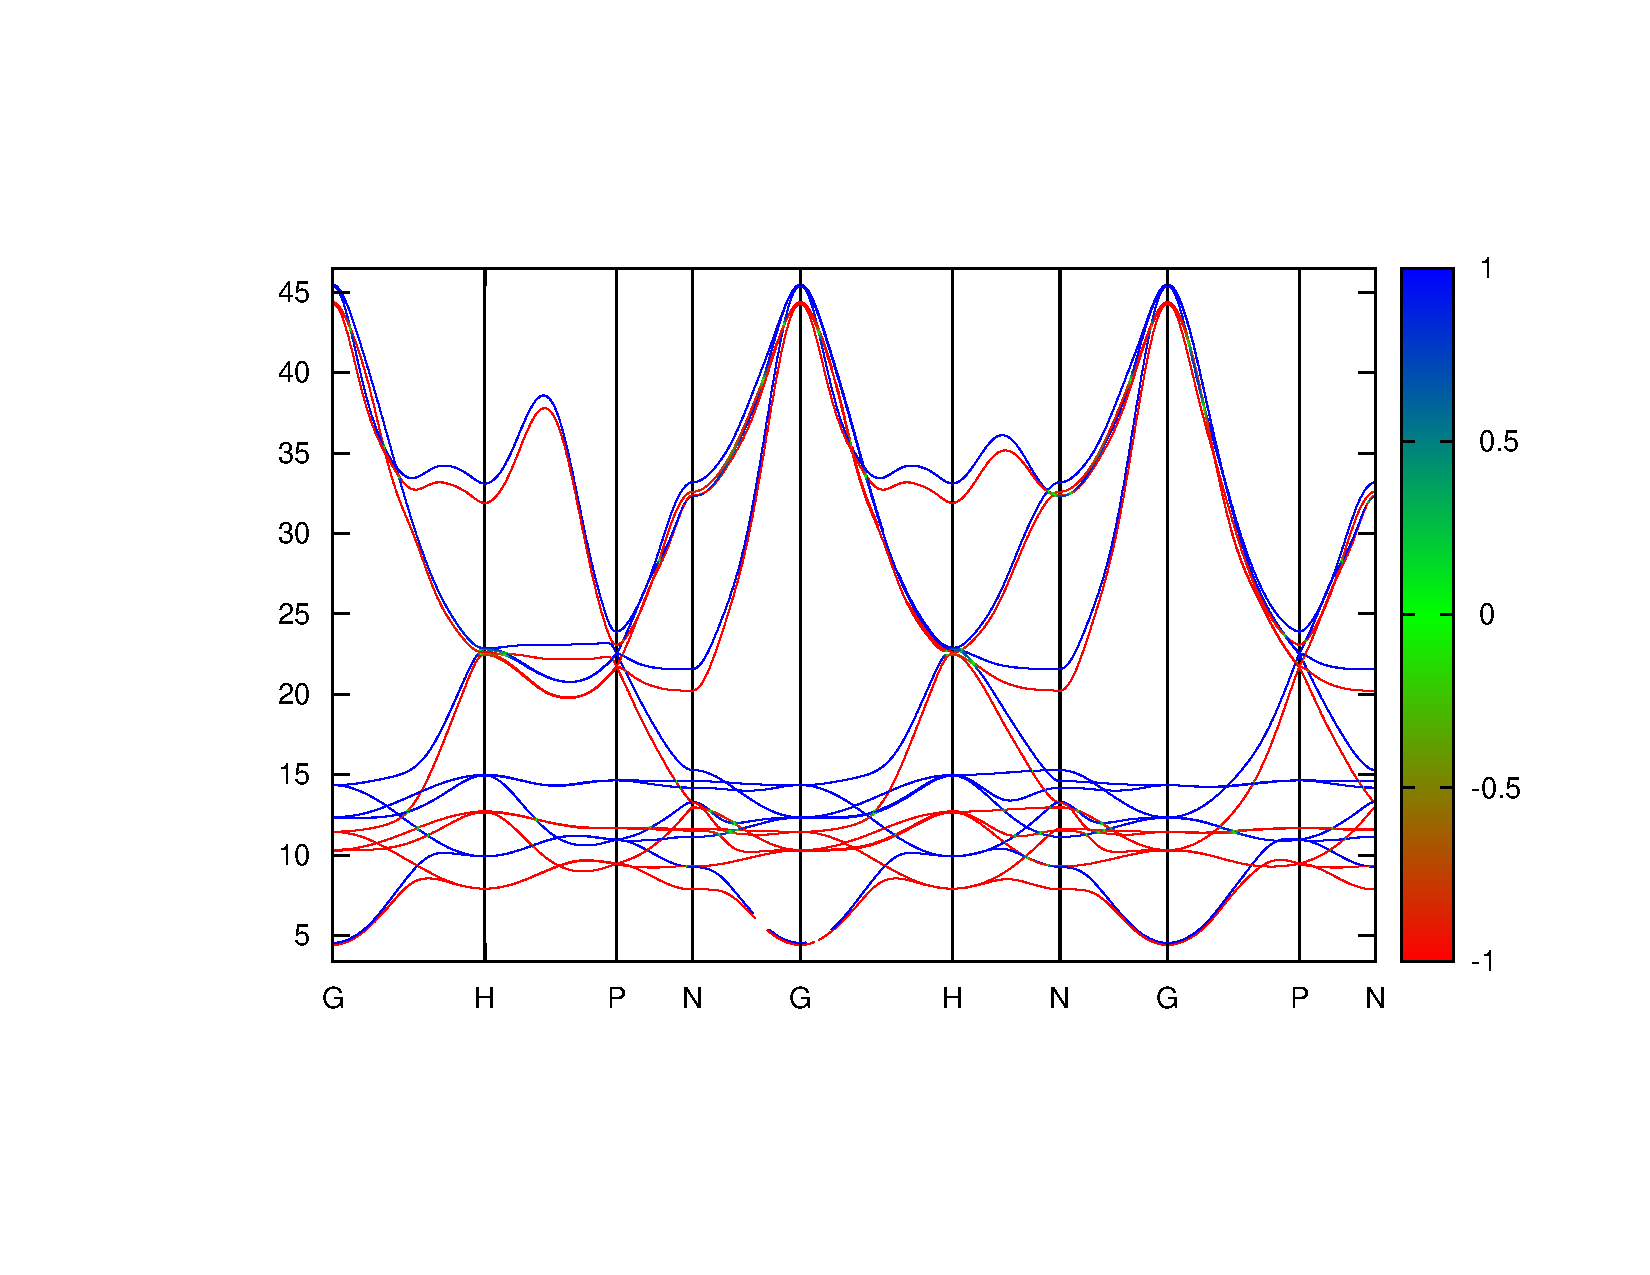
\includegraphics[width=12cm]{Fe_bands}
\caption{Relativistic bandstructure of bcc iron with the magnetization
  along the positive [001] direction. Majority bands (with $\langle
  S_z\rangle=-\hbar/2$) are in red, minority bands ($\langle
  S_z\rangle =+\hbar/2$) in blue. Because of spin-orbit coupling $S_z$
  is not a good quantum number, and intermediate colors occur in the
  vicinity of (avoided) crossings between up- and down-spin bands.
  The Fermi level is at 12.6~eV.}
\label{fig:fe-bnd}
\end{center}
\end{figure}


A suitable path is
{\tt
\begin{quote}
begin kpoint\_path

G 0.0000 0.0000 0.0000   H 0.500 -0.5000 -0.5000

H 0.500 -0.5000 -0.5000  P 0.7500 0.2500 -0.2500

P 0.7500 0.2500 -0.2500  N 0.5000 0.0000 -0.5000

N 0.5000 0.0000 -0.5000  G 0.0000 0.0000 0.000

G 0.0000 0.0000 0.000    H 0.5 0.5 0.5

H 0.5 0.5 0.5            N 0.5 0.0 0.0

N 0.5 0.0 0.0            G 0.0 0.0 0.0

G 0.0 0.0 0.0            P 0.75 0.25 -0.25

P 0.75 0.25 -0.25        N 0.5 0.0 0.0

end kpoint\_path
\end{quote} }

To plot the spin-colored bandstructure using gnuplot (version 4.2 or
higher), issue
{\tt
\begin{quote}
myshell> gnuplot

gnuplot> load `Fe-band.gnu'
\end{quote} }

We can also inspect the constant-energy surfaces across an entire
plane, using the module {\tt kslice}.  To obtain the energy
eigenvalues on a $200\times 200$ grid covering the (010) plane in the
BZ, uncomment the following instructions in {\tt Fe.win}, {\tt
\begin{quote}
kslice = T

kslice\_task = energy\_cntr

kslice\_cntr\_energy = 12.6285

kslice\_interp\_mesh = 200 200

kslice\_corner = 0.0  0.0  0.0

kslice\_b1 =     0.5 -0.5 -0.5

kslice\_b2 =     0.5  0.5  0.5
\end{quote} }

\begin{figure}[h]
\begin{center}
\scalebox{0.85}{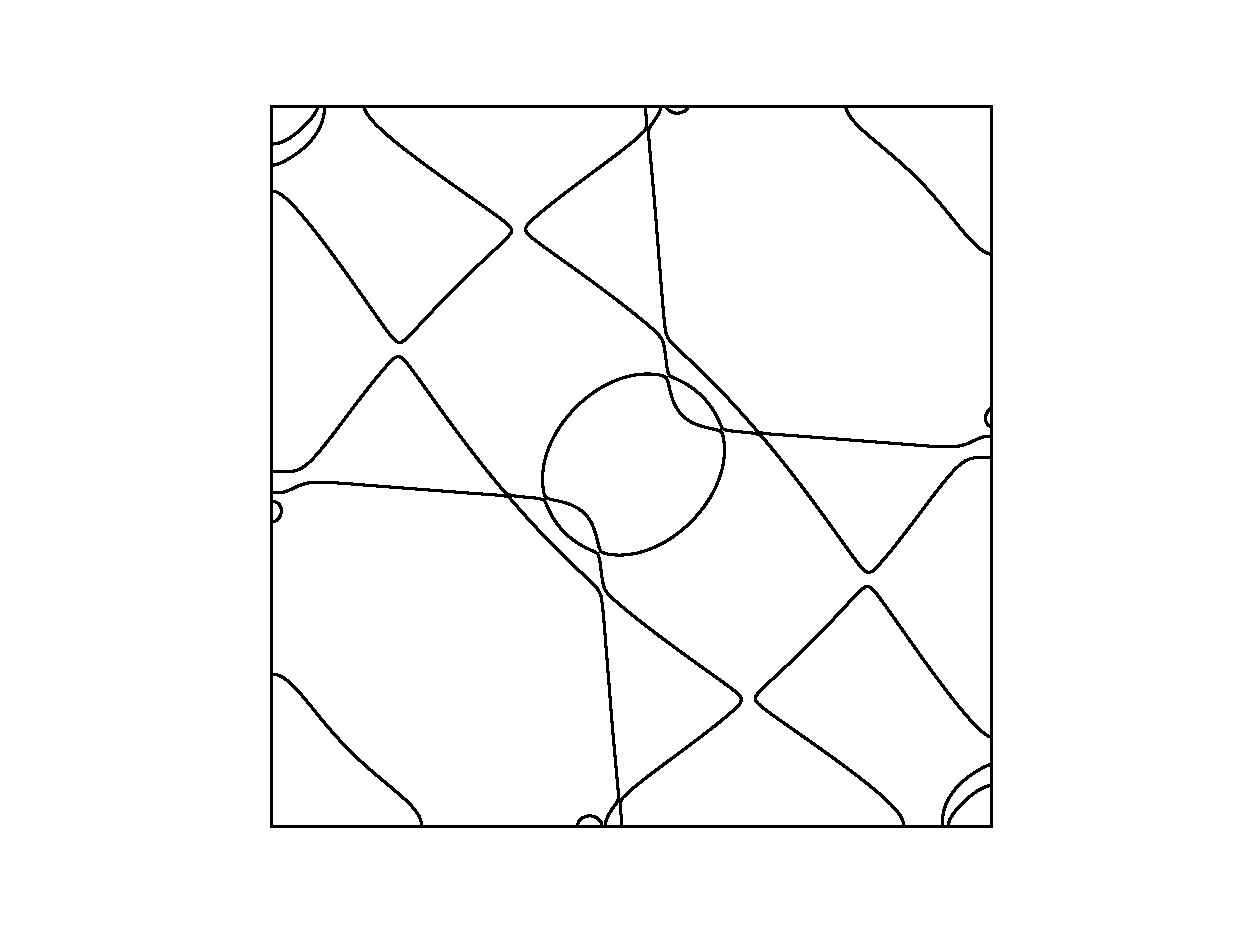
\includegraphics[width=6.5cm]{Fe_fermicontours}}
\caption{Fermi-surface contours on the (010) plane of bcc Fe.} 
\label{fig:fe-fermicontours}
\end{center}
\end{figure}

where we chose the Fermi energy 12.6285~eV (taken from {\tt scf.out})
as the energy level for the isocontours.  The Fermi-surface contours
(lines of intersection between the Fermi surface and the slice), can
be visualized with the script {\tt Fe-energy\_cntr.gnu} generated at
runtime,
%
{\tt
\begin{quote}
myshell> gnuplot

gnuplot> load `Fe-energy\_cntr.gnu'
\end{quote} }
%
(Do not be concerned by the warning messages, they are caused by the
fact that not all bands cross the Fermi energy.) Alternative, one can
use the python script {\tt Fe-energy\_cntr.py} that is also generated
at runtime,
%
{\tt
\begin{quote}
myshell> python Fe-energy\_cntr.py
\end{quote} }


%{\tt
%  octave} script {\tt bands.m}, 
%{\tt
%\begin{quote}
%myshell> octave
%
%octave:1> bands
%\end{quote} }
%\smallskip 

%or with the {\tt python+pylab+numpy} script {\tt bands.py},
%{\tt
%\begin{quote}
%myshell> python bands.py
%\end{quote} }


\subsection*{Further ideas}

\begin{itemize}

%\item Plot the energy bands over a single line segment in $k$-space,
%  e.g., $\Gamma$--H, to see in detail a spin-orbit-induced avoided
%  crossing between majority and minority bands. [Hint: When using {\tt
%    gnuplot} you can zoom in by right-clicking to select a region of
%  the plot.]

\item Generate the Fermi-surface contours on the (001) plane
perpendicular to the magnetization. Note the higher symmetry compared
to Fig.~\ref{fig:fe-fermicontours}.

\item Redraw the Fermi-surface contours on the (010) plane starting
  from an {\it ab initio} calculation without spin-orbit coupling (as
  in Example~8). Note how the connectivity of the Fermi contours
  changes.

\end{itemize}

\cleardoublepage

\section*{18: Iron -- Berry curvature and anomalous Hall 
conductivity}

\begin{itemize}
\item{Outline: \it{Calculate the $k$-space Berry curvature and
      anomalous Hall conductivity by Wannier interpolation, as
      described in Ref.~\cite{wang-prb06}.}}
\item{Directory: {\tt examples/example18/}}
\item{Input files}
\begin{itemize}
\item{ {\tt Fe.scf} {\it The \pwscf\ input file for ground state
    calculation}}
\item{ {\tt Fe.nscf}  {\it The \pwscf\ input file to obtain Bloch
    states on a uniform grid}} 
\item{ {\tt Fe.pw2wan}  {\it The input file for {\tt pw2wannier90}}}
\item{ {\tt Fe.win}  {\it The {\tt wannier90} and {\tt postw90} input file}}
\end{itemize}
\end{itemize}

The sequence of steps below is the same of Example~17.  If you have
already run that example, you can reuse the output files from steps
1--5, and only step 6 must be carried out again using the new input
file {\tt Fe.win}.

\begin{enumerate}
\item Run \pwscf\ to obtain the ground state of iron\\
{\tt pw.x < Fe.scf > scf.out}

\item Run \pwscf\ to obtain the Bloch states on a uniform k-point
  grid\\ 
{\tt pw.x < Fe.nscf > nscf.out}

\item Run \wannier\ to generate a list of the required overlaps (written
  into the {\tt Fe.nnkp} file).\\
{\tt wannier90.x -pp Fe}

\item Run {\tt pw2wannier90} to compute the overlaps between Bloch
  states and the projections for the starting guess (written in the
  {\tt Si.mmn} and {\tt  Si.amn} files).\\
{\tt pw2wannier90.x < Fe.pw2wan > pw2wan.out}

\item Run \wannier\ to compute the MLWF.\\
{\tt wannier90.x Fe}

\item Run \postw\ to compute the Berry curvature.\\
  {\tt postw90.x Fe} (serial execution)\\
  {\tt mpirun -np 8 postw90.x Fe} (parallel execution)


\end{enumerate}

The  Berry curvature of a Bloch state $\psi_{n{\bf k}}=e^{i{\bf k}\cdot {\bf r}}u_{n{\bf k}}$ is a vector property defined as
$$
\bm{\Omega}_n({\bf k})=-{\rm Im}
\langle \bm{\nabla}_{\bf k} u_{n{\bf k}}\vert \times
\vert\bm{\nabla}_{\bf k} u_{n{\bf k}}\rangle.
$$
%
We are interested in the sum over occupied states,
$$
\bm{\Omega}({\bf k})=\sum_n^{\rm occ}\,\bm{\Omega}_n({\bf k}).
$$
%
The following instructions in {\tt Fe.win} are used to calculate
$-\bm{\Omega}({\bf k})$ along lines in $k$-space, 
{\tt
\begin{quote}
fermi\_energy = 12.6285

kpath = T

kpath\_task = curv

kpath\_num\_points=1000
\end{quote} }

The path specification in {\tt Fe.win} is the same as in Example~17,
and the value of the Fermi energy, 12.6285~eV, was taken from {\tt
  scf.out}. 

Carry out the calculation by executing {\tt postw90} (step 6
above). To plot the $z$ component $-\Omega^z({\bf k})$, use the {\tt
  gnuplot} script {\tt Fe-curv\_z.gnu} generated at runtime, 
{\tt
\begin{quote}
myshell> gnuplot

gnuplot> load `Fe-curv\_z.gnu'
\end{quote} }

(compare with Fig.~2 of Ref.~\cite{yao-prl04}).  You can similarly
plot the $x$ and $y$ components.

In Example~17 we plotted the Fermi-surface contours on the (010) plane
in $k$-space.  To add on top a heatmap plot of
$-\bm{\Omega}({\bf k})$, uncomment the following instructions in {\tt
  Fe.win}, \smallskip {\tt
\begin{quote}
kslice = T

kslice\_task = energy\_cntr+curv\_heatmap

kslice\_interp\_mesh = 200

kslice\_corner = 0.0  0.0  0.0

kslice\_b1 =     0.5 -0.5 -0.5

kslice\_b2 =     0.5  0.5  0.5
\end{quote} }
%
and re-run {\tt postw90}.  For the visualization we use the three {\tt
  python} scripts generated at runtime. To plot the $z$ component
$-\Omega^z({\bf k})$, for example, issue
%
{\tt
\begin{quote}
myshell> python Fe-curv\_z-heatmap.py
\end{quote} }
\smallskip

Compare the plot with Fig.~3 in Ref.~\cite{yao-prl04}.

The intrinsic anomalous Hall conductivity (AHC) $\sigma^{\rm
  AH}_{\alpha\beta}=-\sigma^{\rm AH}_{\beta\alpha}$ is proportional to
the integral of the Berry curvature over the entire Brillouin zone.
To evaluate the AHC using a $25\times 25\times 25$ $k$-point mesh,
uncomment the following lines in {\tt Fe.win}, 
{\tt
\begin{quote}
berry = T

berry\_task = ahc                

berry\_interp\_mesh = 25 25 25

\end{quote} } 
(the last instruction can be simplified to {\tt
berry\_interp\_mesh = 25}) and re-run {\tt postw90}.  The AHC in S/cm
is written in the output file {\tt Fe.wpout} in (pseudo)vector
form. The $x$, $y$, and $z$ components correspond to $\sigma^{\rm
  AH}_{yz}$, $\sigma^{\rm AH}_{zx}$, and $\sigma^{\rm AH}_{xy}$
respectively. For bcc Fe with the magnetization along [001], only the
last component is nonzero.
%(the tiny values of the other two components are numerical noise).

\begin{figure}[h]
\begin{center}
\scalebox{0.5}{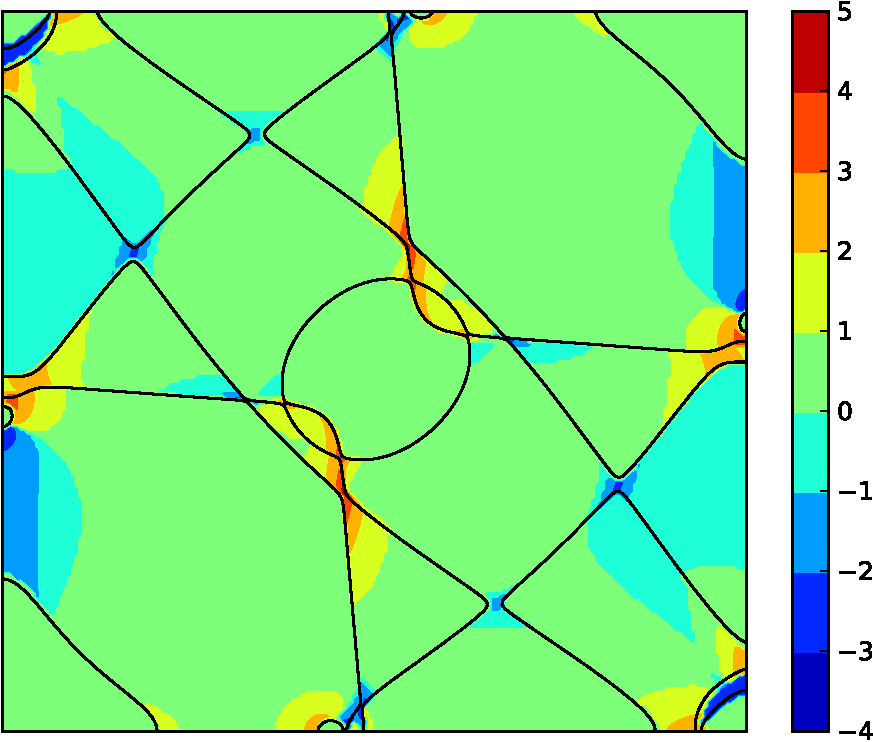
\includegraphics{Fe_curvbands}}
\caption{Berry curvature $-\Omega^z({\bf k})$ on the (010) plane of
  bcc Fe, in atomic units.  The color scale is as follows:
  a positive value, e.g., 2, means $10^2$~bohr$^2$, while a negative value,
  e.g., -2, means $-10^2$~bohr$^2$.}
\label{fig:fe-curv-slice}
\end{center}
\end{figure}

\subsection*{Further ideas}

%\begin{itemize}
%\item 
Study the convergence of the AHC with respect to the density of
  the integration mesh:

  \begin{itemize}

  \item[{\bf --}] Increase the mesh density uniformly by changing {\tt
      berry\_interp\_mesh}.

  \item[{\bf --}] In addition, it helps to adaptively refine the mesh
    in regions where the Berry curvature is large and rapidly varying
    (such regions can be seen in Fig.~\ref{fig:fe-curv-slice}).  Add
    to {\tt Fe.win} the lines \smallskip {\tt
      \begin{quote}
        berry\_adaptive\_mesh = 5  
        
        berry\_adaptive\_thresh = 27.98
      \end{quote} }
    
    in order to interpose a $5\times 5\times 5$ fine mesh around those
    points where $\vert\Omega^z({\bf k})\vert$ exceeds
    27.98~\AA$^2\simeq 100$~bohr$^2$. The percentage of points
    triggering adaptive refinement is given in {\tt Fe.wpout}.

  \item[{\bf --}] Compare the converged AHC value with those reported
    in Refs.~\cite{wang-prb06} and~\cite{yao-prl04}.

  \end{itemize}

% ADD EVENTUALLY? AS A SEPARATE EXAMPLE?
%
%\item The Berry curvature in ferromagnets results from broken
%  time-reversal in the orbital wavefunctions, induced by the magnetic
%  order combined with spin-orbit coupling. Another source of Berry
%  curvature in crystals is lack of spatial inversion symmetry.
%
%  Plot the Berry curvature of the valence bands of GaAs along selected
%  lines and planes in the BZ. Note that $\bm{\Omega}(-{\bf
%    k})=-\bm{\Omega}({\bf k})$, so that $\int_{\rm
%    BZ}\bm{\Omega}({\bf k})d{\bf k}=0$.
  


%\end{itemize}


\cleardoublepage

\section*{19: Iron -- Orbital magnetization}


\begin{itemize}
\item{Outline: \it{Calculate the bulk orbital magnetization by Wannier
      interpolation, as described in Ref.~\cite{lopez-prb12}.}}
\item{Directory: {\tt examples/example19/}}
\item{Input files}
\begin{itemize}
\item{ {\tt Fe.scf} {\it The \pwscf\ input file for ground state
    calculation}}
\item{ {\tt Fe.nscf}  {\it The \pwscf\ input file to obtain Bloch
    states on a uniform grid}} 
\item{ {\tt Fe.pw2wan}  {\it The input file for {\tt pw2wannier90}}}
\item{ {\tt Fe.win}  {\it The {\tt wannier90} and {\tt postw90} input file}}
\end{itemize}
\end{itemize}

The sequence of steps below is the same of Examples~17 and 18.  If you
have already run one of those examples, you can reuse the output files
from steps 1--3 and 5. Steps~4 and 6 should be carried out again using
the new input files {\tt Fe.pw2wan} and {\tt Fe.win}.

\begin{enumerate}
\item Run \pwscf\ to obtain the ground state of iron\\
{\tt pw.x < Fe.scf > scf.out}

\item Run \pwscf\ to obtain the Bloch states on a uniform k-point
  grid\\ 
{\tt pw.x < Fe.nscf > nscf.out}

\item Run \wannier\ to generate a list of the required overlaps (written
  into the {\tt Fe.nnkp} file).\\
{\tt wannier90.x -pp Fe}


\item Run {\tt pw2wannier90} to compute:
  \begin{itemize}

  \item[{\bf --}] The overlaps $\langle u_{n{\bf k}}\vert u_{m{\bf k}+{\bf
          b}}\rangle$ (written in the {\tt Fe.mmn} file)

  \item[{\bf --}] The projections for the starting guess (written in the {\tt
        Fe.amn} file)

  \item[{\bf --}] The matrix elements $\langle u_{n{\bf k}+{\bf b}_1}\vert
      H_{\bf k}\vert u_{m{\bf k}+{\bf b}_2}\rangle$ (written in the
      {\tt Fe.uHu} file)

  \item[{\bf --}] The spin matrix elements $\langle \psi_{n{\bf
        k}}\vert \sigma_i\vert \psi_{m{\bf k}}\rangle$ (written in the
    {\tt Fe.spn} file)

  \end{itemize}
{\tt pw2wannier90.x < Fe.pw2wan > pw2wan.out}

\item Run \wannier\ to compute the MLWF.\\
{\tt wannier90.x Fe}

\item Run \postw\ to compute the orbital magnetization.\\
  {\tt postw90.x Fe} (serial execution)\\
  {\tt mpirun -np 8 postw90.x Fe} (parallel execution)


\end{enumerate}

The orbital magnetization is computed in the {\tt berry} module of
{\tt postw90} as the BZ integral of a quantity ${\bf M}_{\rm orb}({\bf
  k})$ similar to the Berry curvature (see Ref.~\cite{lopez-prb12} for
its definition) \tent{{\bf [eventually refer instead to the yet-to-be-written
description of the {\tt berry} module in the user guide]}}, 
%
{\tt
\begin{quote}
berry = T

berry\_task = morb

berry\_interp\_mesh = 25 25 25

\end{quote} }

As in the case of the AHC, it is necessary to specify the Fermi level
in order to compute ${\bf M}_{\rm orb}$,
%
{\tt
\begin{quote}
fermi\_energy = 12.6285
\end{quote}
} 
%
Compare the value of the orbital magnetization in {\tt Fe.wpout} with
the spin magnetization in {\tt scf.out}.\footnote{Alternatively, the
spin magnetization can be computed by {\tt postw90}. This requires adding the
instruction {\tt spn\_moment = T} to {\tt Fe.win}, assuming that {\tt pw2wannier90}
was executed with {\tt write\_spn = .true.} in {\tt Fe.pw2wan}.} 
Both point along $\hat{\bf
  z}$, but the orbital contribution is much smaller (it is strongly
quenched by the crystal field).

Similarly to the AHC in Example~18, the distribution of the orbital
magnetization in $k$-space can be visualized by plotted along lines or
planes in the BZ.  To plot $M^z_{\rm orb}({\bf k})$ along
high-symmetry lines, uncomment in {\tt Fe.win} the block of
instructions containing {\tt
\begin{quote}
kpath\_task = morb
\end{quote}
}
After running {\tt postw90}, do
{\tt
\begin{quote}
myshell> gnuplot

gnuplot> load `Fe-bands.gnu'

gnuplot> load `Fe-morb\_z.gnu'
\end{quote} }
Compare the two plots with Fig.~2 of Ref.~\cite{lopez-prb12}.


To plot $M^z_{\rm orb}({\bf k})$ together with the Fermi contours on the
(010) BZ plane, uncomment in {\tt
  Fe.win} the block of instructions containing 
{\tt
\begin{quote}
kslice\_task = energy\_cntr+morb\_heatmap
\end{quote}
} 
re-run {\tt postw90}, and issue
{\tt
\begin{quote}
myshell> python Fe-morb\_z-heatmap.py
\end{quote} } The orbital magnetization is more evenly distributed in
$k$-space than the AHC (Fig.~\ref{fig:fe-curv-slice}), and therefore
converges more rapidly with the number of $k$-points used to sample
the BZ.



\cleardoublepage

\section*{20: Iron -- Optical conductivity and joint density-of-states}

\begin{itemize}
\item{Outline: \it{Calculate the joint density-of-states (JDOS) and
      interband optical conductivity by Wannier interpolation, as
      described in Ref.~\cite{WanInt}.}}
\item{Directory: {\tt examples/example20/}}
\item{Input files}
\begin{itemize}
\item{ {\tt Fe.scf} {\it The \pwscf\ input file for ground state
    calculation}}
\item{ {\tt Fe.nscf}  {\it The \pwscf\ input file to obtain Bloch
    states on a uniform grid}} 
\item{ {\tt Fe.pw2wan}  {\it The input file for {\tt pw2wannier90}}}
\item{ {\tt Fe.win}  {\it The {\tt wannier90} and {\tt postw90} input file}}
\end{itemize}
\end{itemize}

The sequence of steps below is the same of Examples~17--19.  If you
have already run one of those examples, you can reuse the output files
from steps 1--5, and only step 6 must be carried out again using the
new input file {\tt Fe.win}.

\begin{enumerate}
\item Run \pwscf\ to obtain the ground state of iron\\
{\tt pw.x < Fe.scf > scf.out}

\item Run \pwscf\ to obtain the Bloch states on a uniform k-point
  grid\\ 
{\tt pw.x < Fe.nscf > nscf.out}

\item Run \wannier\ to generate a list of the required overlaps (written
  into the {\tt Fe.nnkp} file).\\
{\tt wannier90.x -pp Fe}

\item Run {\tt pw2wannier90} to compute:
  \begin{itemize}

  \item[{\bf --}] The overlaps $\langle u_{n{\bf k}}\vert u_{m{\bf k}+{\bf
          b}}\rangle$ (written in the {\tt Fe.mmn} file)

  \item[{\bf --}] The projections for the starting guess (written in the {\tt
        Fe.amn} file)

  \item[{\bf --}] The spin matrix elements $\langle \psi_{n{\bf
        k}}\vert \sigma_i\vert \psi_{m{\bf k}}\rangle$ (written in the
    {\tt Fe.spn} file)\footnote{These are only used in connection with
{\tt spn\_decomp} in ``Further ideas.''}

  \end{itemize}
{\tt pw2wannier90.x < Fe.pw2wan > pw2wan.out}

\item Run \wannier\ to compute the MLWF.\\
{\tt wannier90.x Fe}

\item Run \postw\ to compute the JDOS and optical conductivity.\\
  {\tt postw90.x Fe} (serial execution)\\
  {\tt mpirun -np 8 postw90.x Fe} (parallel execution)

\end{enumerate}

The following lines in {\tt Fe.win}
%
{\tt
\begin{quote}
berry = T

berry\_interp\_mesh = 25

berry\_task = optics

optics\_energy\_max = 7.0

optics\_time\_parity = even 

\end{quote} }
%
instruct {\tt postw90} to calculate the time-even (symmetric) part
${\rm Re}\,\sigma^{\rm S}_{\alpha\beta}(\omega)={\rm Re}\,\sigma^{\rm
  S}_{\beta\alpha}(\omega)$ of the absorptive optical conductivity
tensor in the range $\omega\in [0,7]$~eV, using a $25^3$ $k$-point
mesh. The JDOS is also calculated over the same spectral
range. Similarly to the AHC (Example~18) and orbital magnetization
(Example~19), the value of the Fermi energy must be specified in {\tt
  Fe.win},
%
{\tt
\begin{quote}
fermi\_energy = 12.6285
\end{quote}
}

To plot the DOS using {\tt gnuplot}, do
%
{\tt
\begin{quote}
myshell> gnuplot

gnuplot> plot `Fe-jdos.dat' w l
\end{quote} }

In general ${\rm Re}\,\sigma^{\rm S}_{\alpha\beta}(\omega)$ has six independent
components, but in bcc Fe only the diagonal components are nonzero. 
To plot ${\rm Re}\,\sigma^{\rm S}_{xx}(\omega)$ with {\tt gnuplot},
use
%
{\tt
\begin{quote} myshell> gnuplot

gnuplot> plot `Fe-sigS\_xx.dat' w l
\end{quote} }
%
(As indicated in {\tt Fe.wpout}, the conductivity is plotted in units
of $10^{15}$~sec$^{-1}$.) The difference in shape between the JDOS and
the optical conductivity can be attributed to the variability in the
dipole matrix elements describing the optical transitions.  Note also
that the calculated spectrum is ``sharp,'' while experimental spectra
are broadened by lifetime effects which are not taken into account in
the calculation.

The optical conductivity tensor of iron also has an antisymmetric
(time-odd) part associated with magneto-optical effects. To calculate
the absorptive part ${\rm Im}\,\sigma^{\rm A}_{\alpha\beta}(\omega)$,
change in {\tt Fe.win},
%
{\tt
\begin{quote}
optics\_time\_parity = odd
\end{quote} }
%
and re-run {\tt postw90}. The only nonzero component is ${\rm
  Im}\,\sigma^{\rm A}_{xy}(\omega)=-{\rm Im}\,\sigma^{\rm
  A}_{yx}(\omega)$.  It describes the differential absorption of left-
anf right-circularly-polarized light travelling along the
magnetization direction $\hat{\bf z}$. To plot this
``magnetic circular dichroism'' (MCD) spectrum, issue
%
{\tt
\begin{quote} myshell> gnuplot

gnuplot> plot `Fe-sigA\_xy.dat' w l
\end{quote} }
%
Following a common convention in the literature, what is plotted is
$\omega{\rm Im}\,\sigma^{\rm A}_{xy}(\omega)$, in units of
$10^{29}$~sec$^{-2}$. Compare the spectrum with the one displayed in
Ref.~\cite{yao-prl04}. To improve the agreement, you need to increase
the number of $k$-points from $25^3$ to, e.g., $125^3$.


\newpage

\subsection*{Further ideas}

\begin{itemize}

\item Recompute the ordinary and dichroic optical conductivities after
  adding to the input file the line
%
{\tt
\begin{quote}

spn\_decomp = T
\end{quote} }
%
This adds three extra columns to the *sig*.dat output files,
containing the breakdown of $\sigma(\omega)$ into
up~$\rightarrow$~up, down~$\rightarrow$~down, and spin-flip
transitions.

\item The MCD spectrum is related to the AHC by a Kramers-Kronig
relation,
%
$$
\sigma^{\rm AH}_{xy}=\frac{2}{\pi}\int_0^\infty\,
\frac{1}{\omega}{\rm Im}\,\sigma^{\rm A}_{xy}(\omega)\,d\omega
$$

This integral is evaluated numerically by {\tt postw90} by replacing
the limits of integration with $\int_{\omega_{\rm min}}^{\omega_{\rm
    max}}$, where $\omega_{\rm max}$ equals {\tt optics\_max\_energy}
and $\omega_{\rm min}$ is scanned in the range $[0,\omega_{\rm
  max}]$. To plot the result (in S/cm) versus $\omega_{\rm min}$, do
%
{\tt
\begin{quote} myshell> gnuplot

gnuplot> plot `Fe-kk\_xy.dat' w l
\end{quote} }
%
Compare the value at $\omega_{\rm min}=0$ with the AHC value
calculated in Example~18 by directly integrating the $k$-space Berry
curvature.

\item ac AHC from Kramers-Kronig \textcolor{red}{TO BE DONE}

\end{itemize}

\cleardoublepage


\begin{thebibliography}{99}

\bibitem{UserGuide} A.~A.~Mostofi and J.~R.~Yates, \wannier: User
  Guide, available at {\tt http://www.wannier.org/user\_guide.html}.
\textcolor{red}{Add Giovanni and Ivo as co-authors?}

\bibitem{MV} N.~Marzari and D.~Vanderbilt, 
  Maximally Localized Generalized Wannier Functions for Composite
  Energy Bands, {\it Phys. Rev. B} {\bf 56}, 12847 (1997).  

\bibitem{SMV} I.~Souza, N.~Marzari and D.~Vanderbilt, Maximally
     Localized Wannier Functions for Entangled Energy Bands, {\it
     Phys. Rev. B} {\bf 65}, 035109 (2001).

\bibitem{W90} A.~A.~Mostofi, J.~R.~Yates, Y.-S.~Lee, I.~Souza,
   D.~Vanderbilt and N.~Marzari, \wannier: A Tool for Obtaining
   Maximally-Localized Wannier Functions, {\it Comput. Phys. Commun.},
   178, 685 (2008) and {\tt http://arxiv.org/abs/0708.0650}.

\bibitem{USPP} D.~Vanderbilt, Soft Self-Consistent Pseudopotentials in
  a Generalized Eigenvalue Formalism, {\it Phys. Rev. B} {\bf 41}
  (11), 7892 (1990).

\bibitem{BaTiO3} N.~Marzari and D.~Vanderbilt, Maximally-Localized
  Wannier Functions in Perovskites: BaTiO$_3$,
  {\tt http://arxiv.org/abs/cond-mat/9802210}.

\bibitem{WanInt} J.~R.~Yates {\it et al.}, Spectral and Fermi
  Surface Properties from Wannier Interpolation, {\it Phys. Rev. B}
  {\bf 75}, 195121 (2007). 

\bibitem{WanTran} Y.-S.~Lee, M.~B.~Nardelli and N.~Marzari, Band
  Structure and Quantum Conductance of Nanostructures from Maximally
  Localized Wannier Functions: The Case of Functionalized Carbon
  Nanotubes, {\it Phys. Rev. Lett.} {\bf 95}, 076804 (2005).

\bibitem{wang-prb06} X.~Wang {\it et al.}, Ab-initio calculation of
  the anomalous Hall conductivity by Wannier interpolation,
{\it Phys. rev. B} {\bf 74}, 195118 (2006).

\bibitem{yao-prl04} Y.~Yao {\it et al.}, First Principles Calculation
  of Anomalous Hall Conductivity in Ferromagnetic bcc Fe,
{\it Phys. Rev. Lett.} {\bf 92}, 037204 (2004).

\bibitem{lopez-prb12} M.~G.~Lopez, D.~Vanderbilt, T.~Thonhauser, and I.~Souza,
Wannier-based calculation of the orbital magnetization in crystals,
Phys. Rev. B {\bf 85}, 014435 (2012).

\end{thebibliography}

\end{document}
